\subsection{Fliesskommazahlen}

\paragraph{Aufgabe \ref{groesste_klein}}
Die grösste Zahl in diesem System ist \(3.5\).
\begin{figure}[H]
\centering
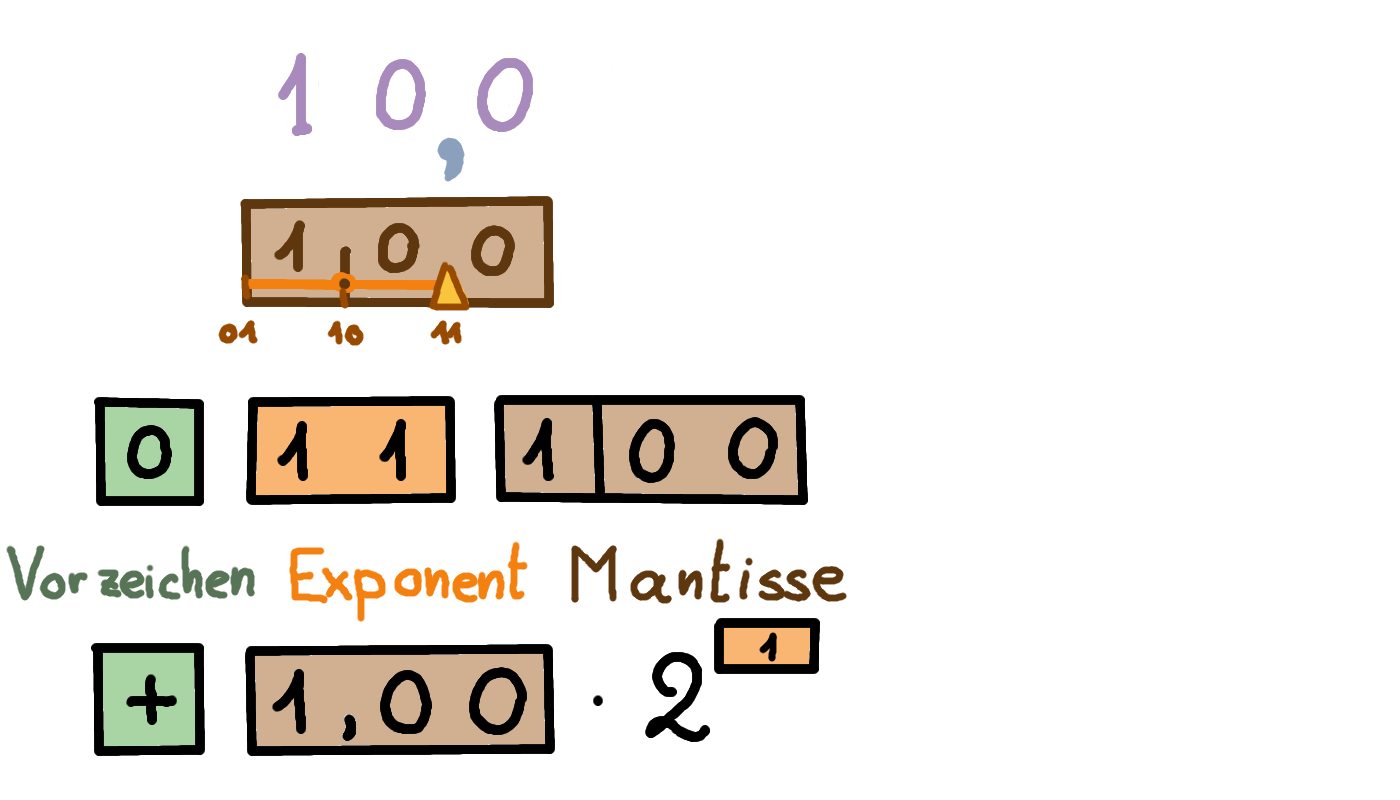
\includegraphics[width=0.65\linewidth]{Pictures/groessteZahl3_klein.png}
\end{figure}

Die kleinste Zahl in diesem System ist \(0.5\).
\begin{figure}[H]
\centering
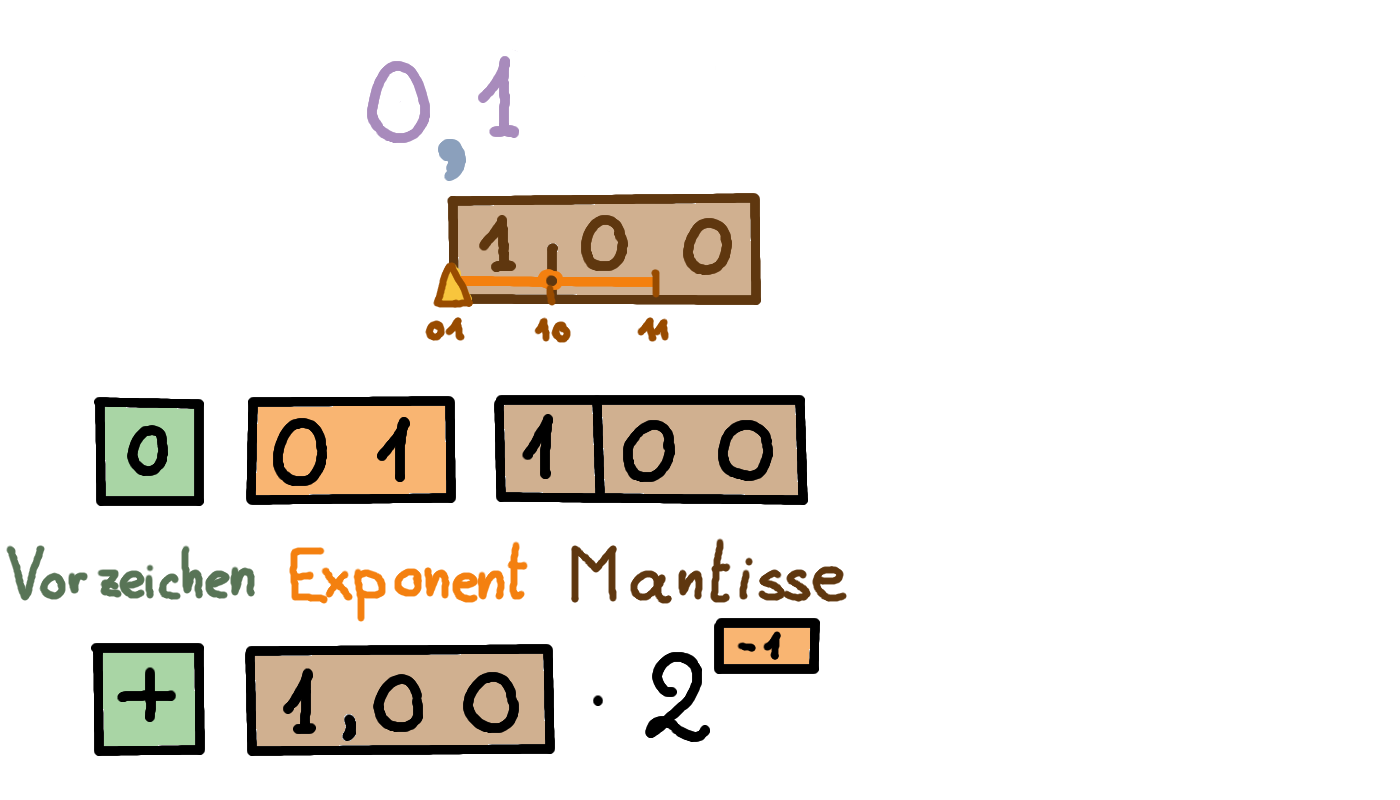
\includegraphics[width=0.65\linewidth]{Pictures/kleinsteZahl3_klein.png}
\end{figure}

%--------------------------------

\paragraph{Aufgabe \ref{nachbarn}}

\begin{enumerate}[(a)]
\item Die Nachbarn von \(2\) sind \(31/16\) und \(17/8\).
\begin{figure}[H]
\centering
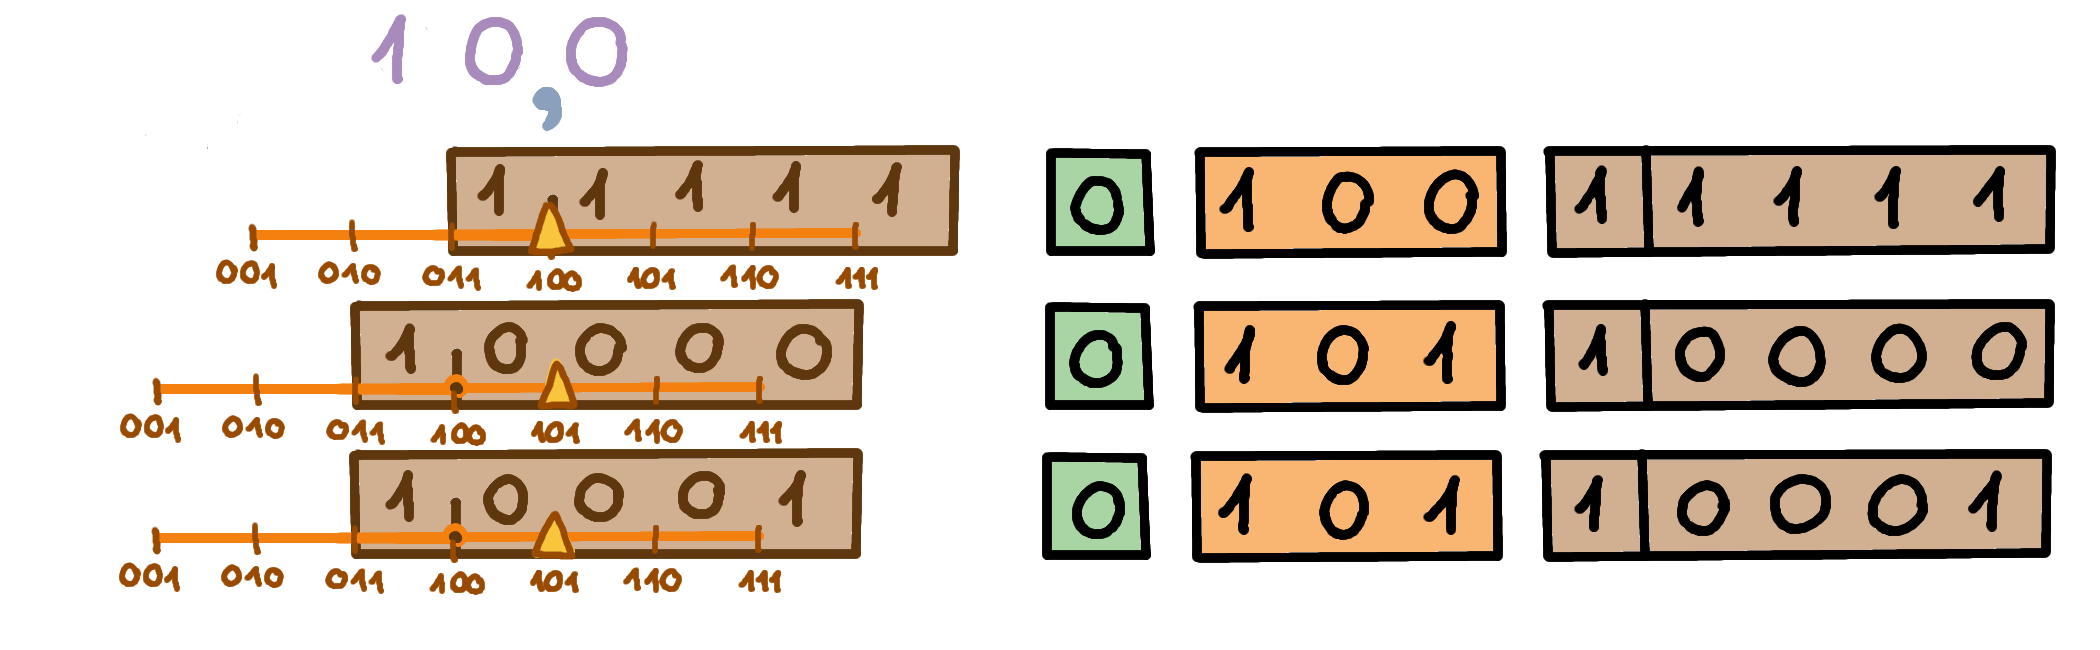
\includegraphics[width=\linewidth]{Pictures/Nachbarn2.png}
\end{figure}

\item Die Nachbarn von \(3\) sind \(23/8\) und \(25/8\).
\begin{figure}[H]
\centering
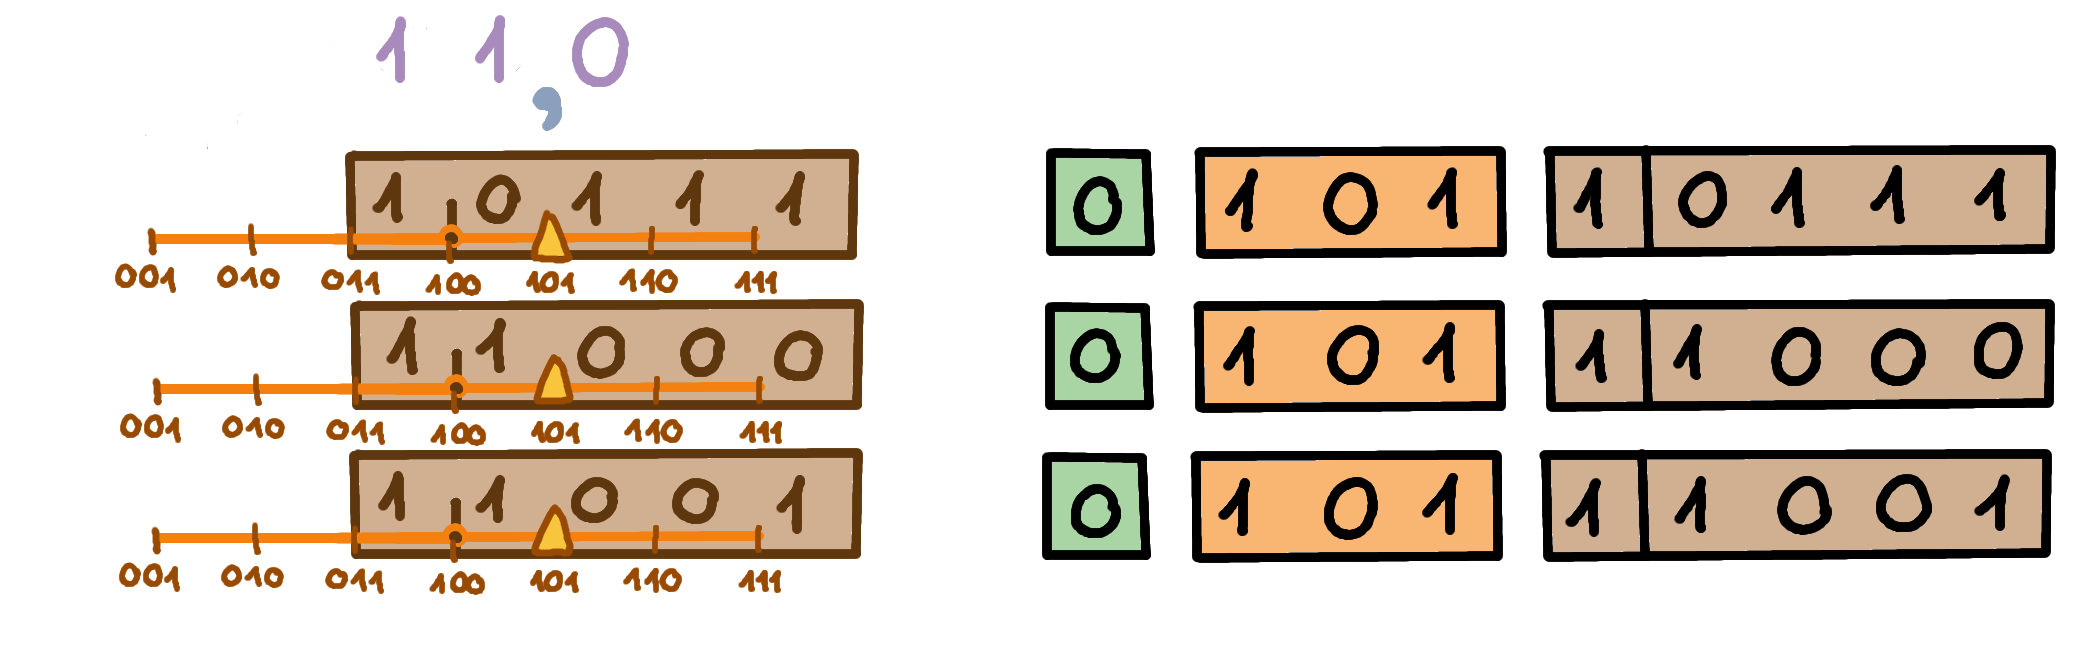
\includegraphics[width=\linewidth]{Pictures/Nachbarn3.png}
\end{figure}

\item Die Nachbarn von \(4\) sind \(31/8\) und \(17/4\).
\begin{figure}[H]
\centering
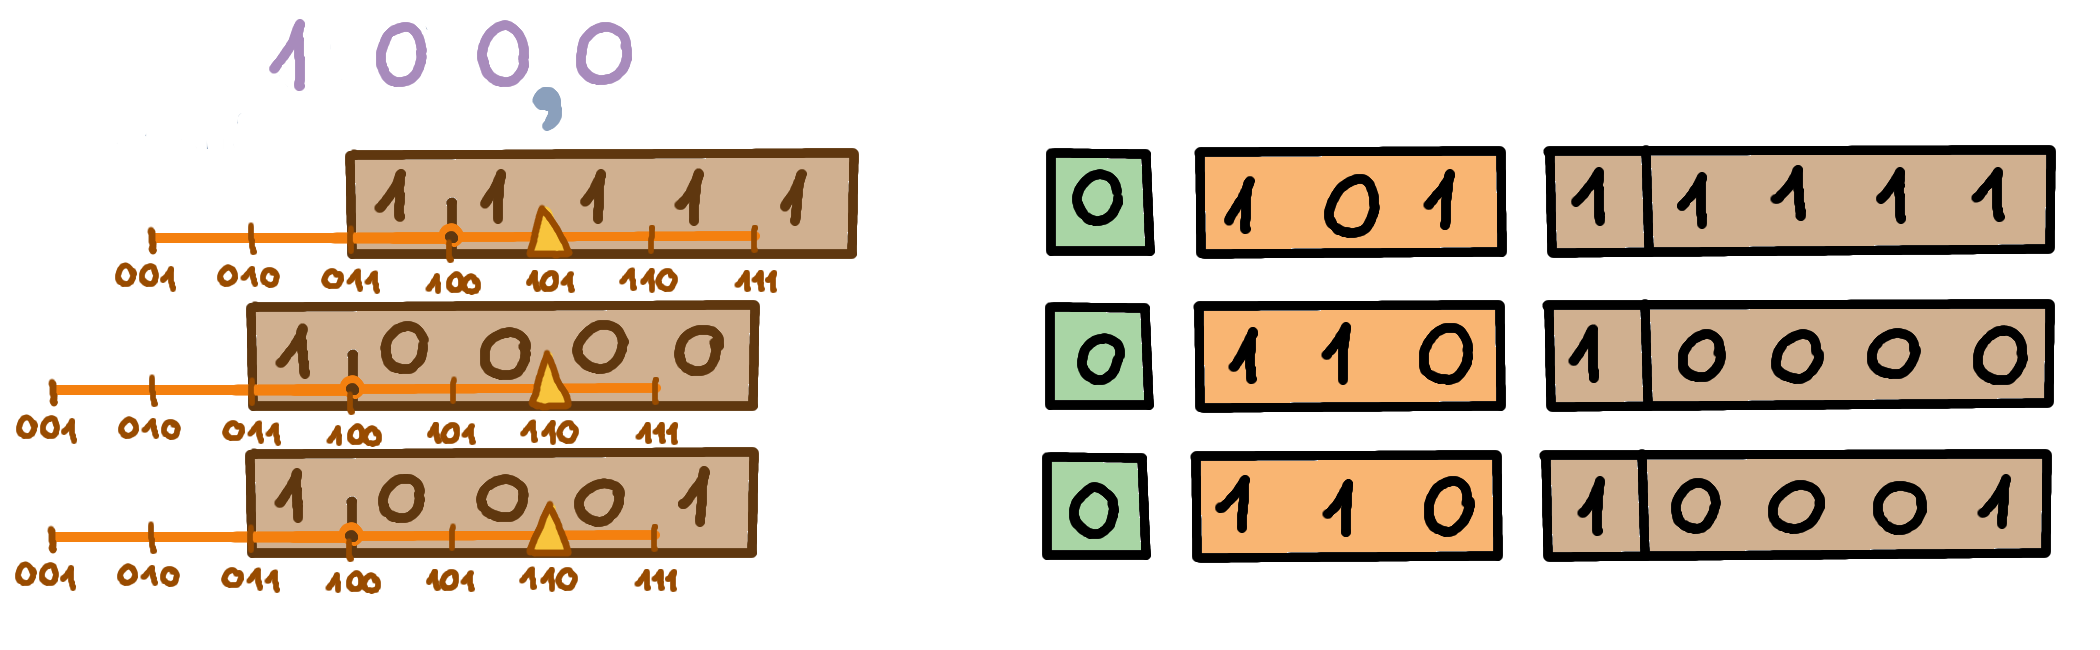
\includegraphics[width=\linewidth]{Pictures/Nachbarn4.png}
\end{figure}

\end{enumerate}

%--------------------------------

\paragraph{Aufgabe \ref{fliesskommazahlen_kontrollfragen}}
\begin{enumerate}[(a)]
\item Nein, es gibt unendlich viele reelle Zahlen und endlich viele Fliesskommazahlen.
\item Ja, die grösste Zahl ist \(1.1111 \ldots 111 \cdot 2^{e_{max}}\).
\item Ja, die kleinste Zahl ist \(1.0000 \ldots 000 \cdot 2^{e_{min}}\).
\item Zum Beispiel, die Zahl \(2.25\) lässt sich in diesem System nicht exakt darstellen.
\item Nein, die darstellbare Fliesskommazahlen sind nicht gleichverteilt. Die kleineren stehen dichter beieinander, weil bei kleineren Zahlen die letzte Stelle der Mantisse weniger Wert ist.
\end{enumerate}

%--------------------------------

\subsection{Addition}
\paragraph{Aufgabe \ref{addition}}
\begin{enumerate}[(a)]
\item \(5/8 + 3/4 = 11/8\), in der Exponentialschreibweise \(1.0110 \cdot 2^{0}\)

Im ersten Schritt schreiben wir die Zahlen auf.
\begin{figure}[H]
\centering
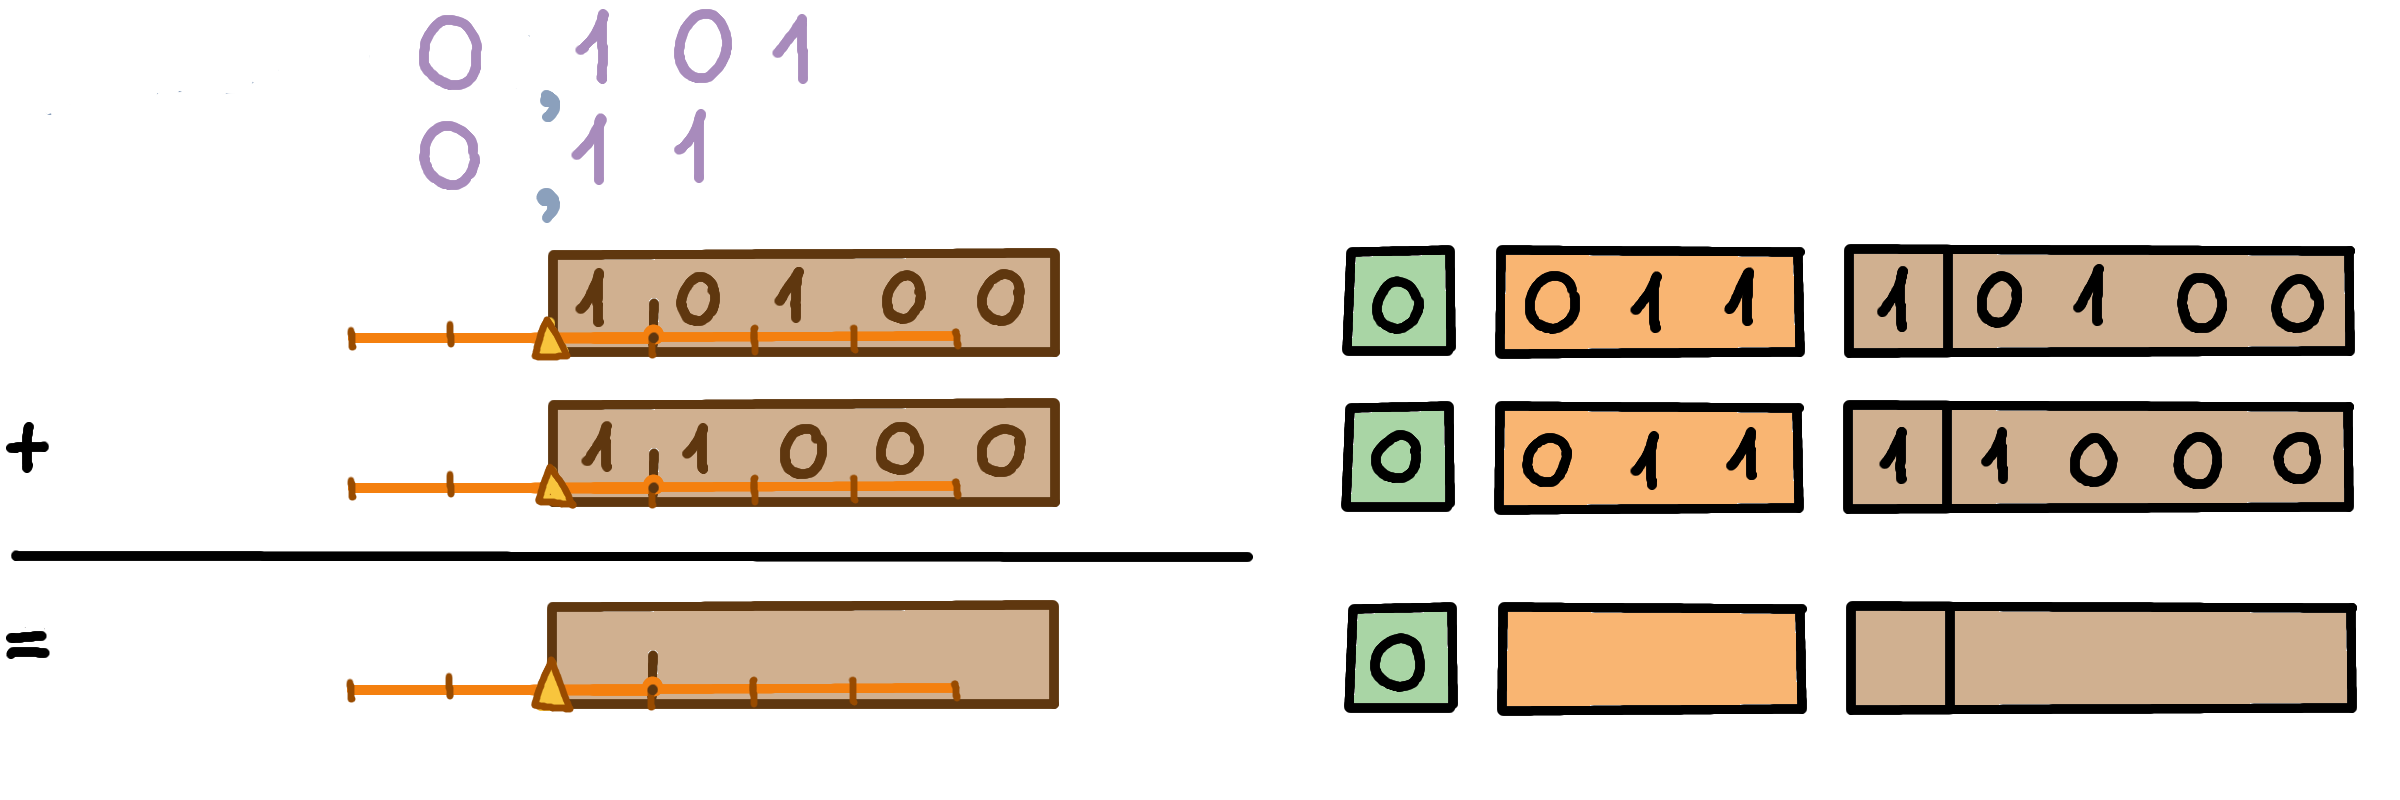
\includegraphics[width=\linewidth]{Pictures/Addition5-8and3-4_1.png}
\end{figure}
Da die zwei Kasten schon übereinander liegen, müssen wir sie nicht verschieben und können die Bits stellenweise zusammen addieren.
\begin{figure}[H]
\centering
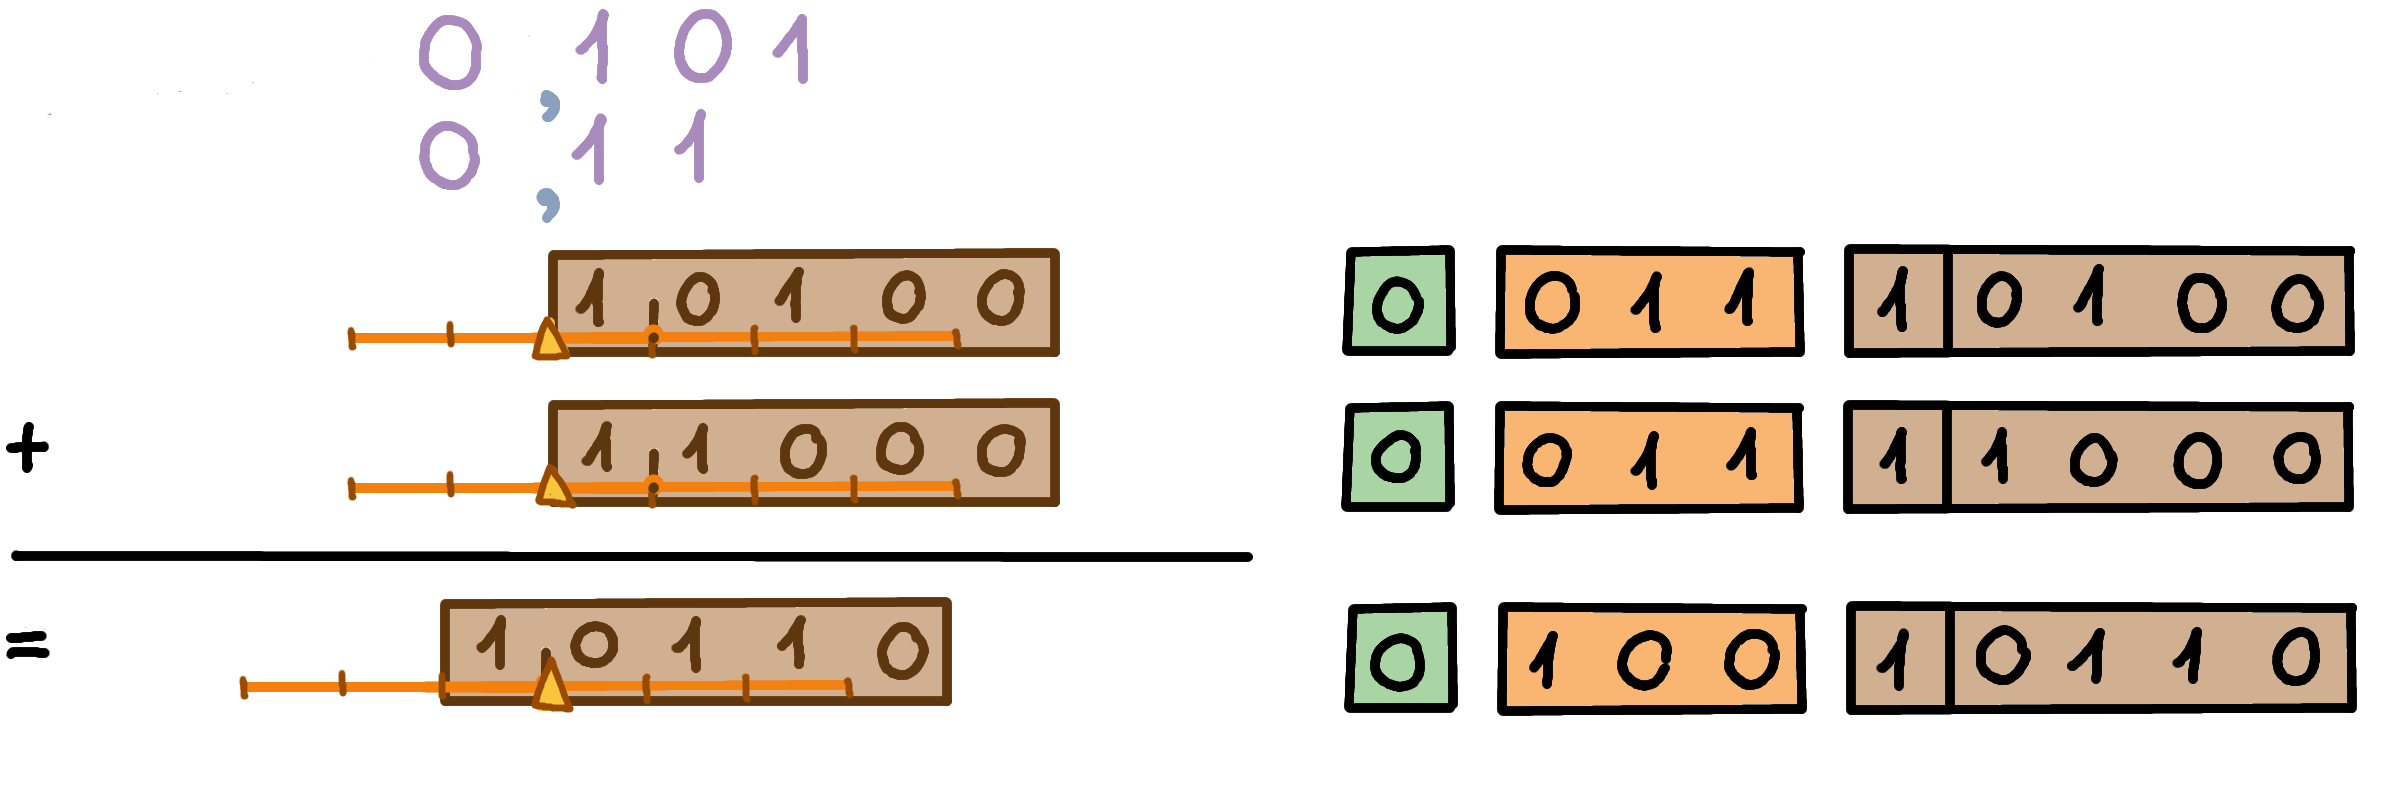
\includegraphics[width=\linewidth]{Pictures/Addition5-8and3-4_2.png}
\end{figure}
Der Kasten vom Ergebnis ist verschoben bezüglich den Kasten der Summanden.

\item \(10 + 2.25 = 12\), in der Exponentialschreibweise \(1.1000 \cdot 2^3\)

Im ersten Schritt schreiben wir die Zahlen auf.
\begin{figure}[H]
\centering
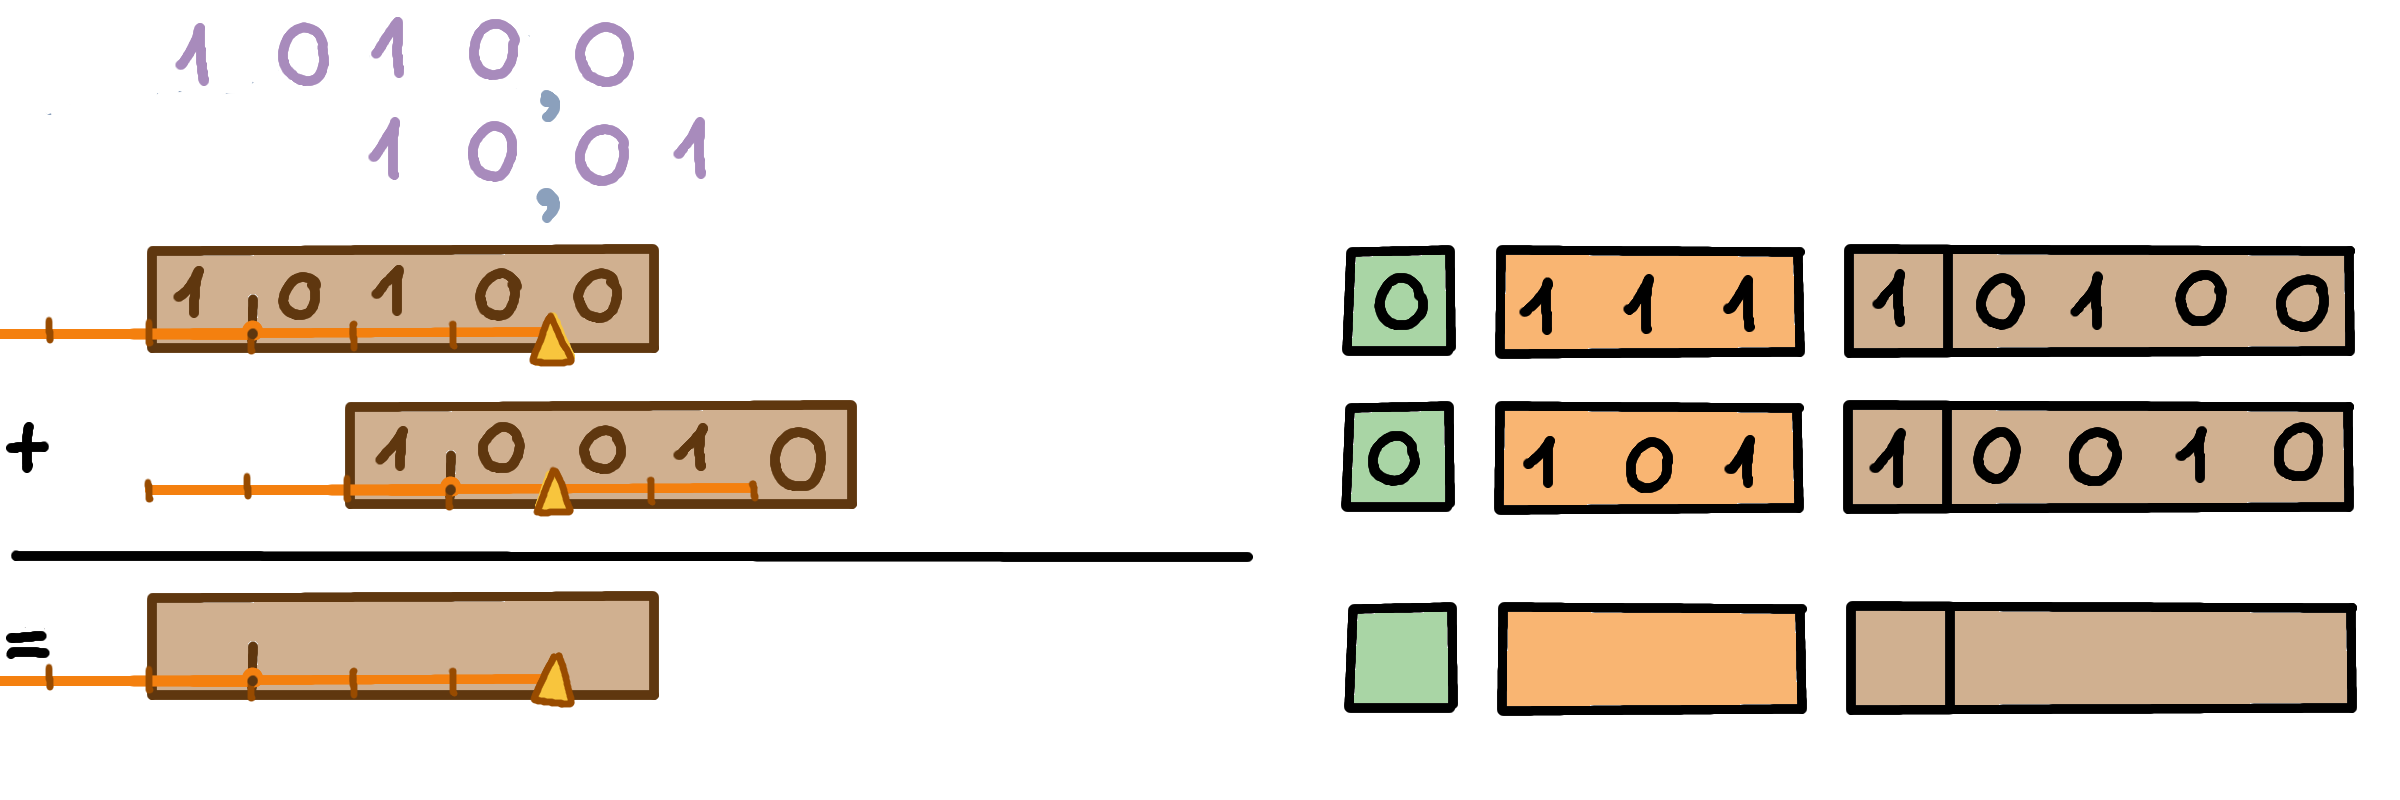
\includegraphics[width=\linewidth]{Pictures/Addition10and2-25_1.png}
\end{figure}

Im zweiten Schritt schiben wir den Kasten von der kleinsten Zahl unter den Kasten der grössten Zahl. Dabei gehen zwei Stellen verloren, eine davon ist eine Eins.
\begin{figure}[H]
\centering
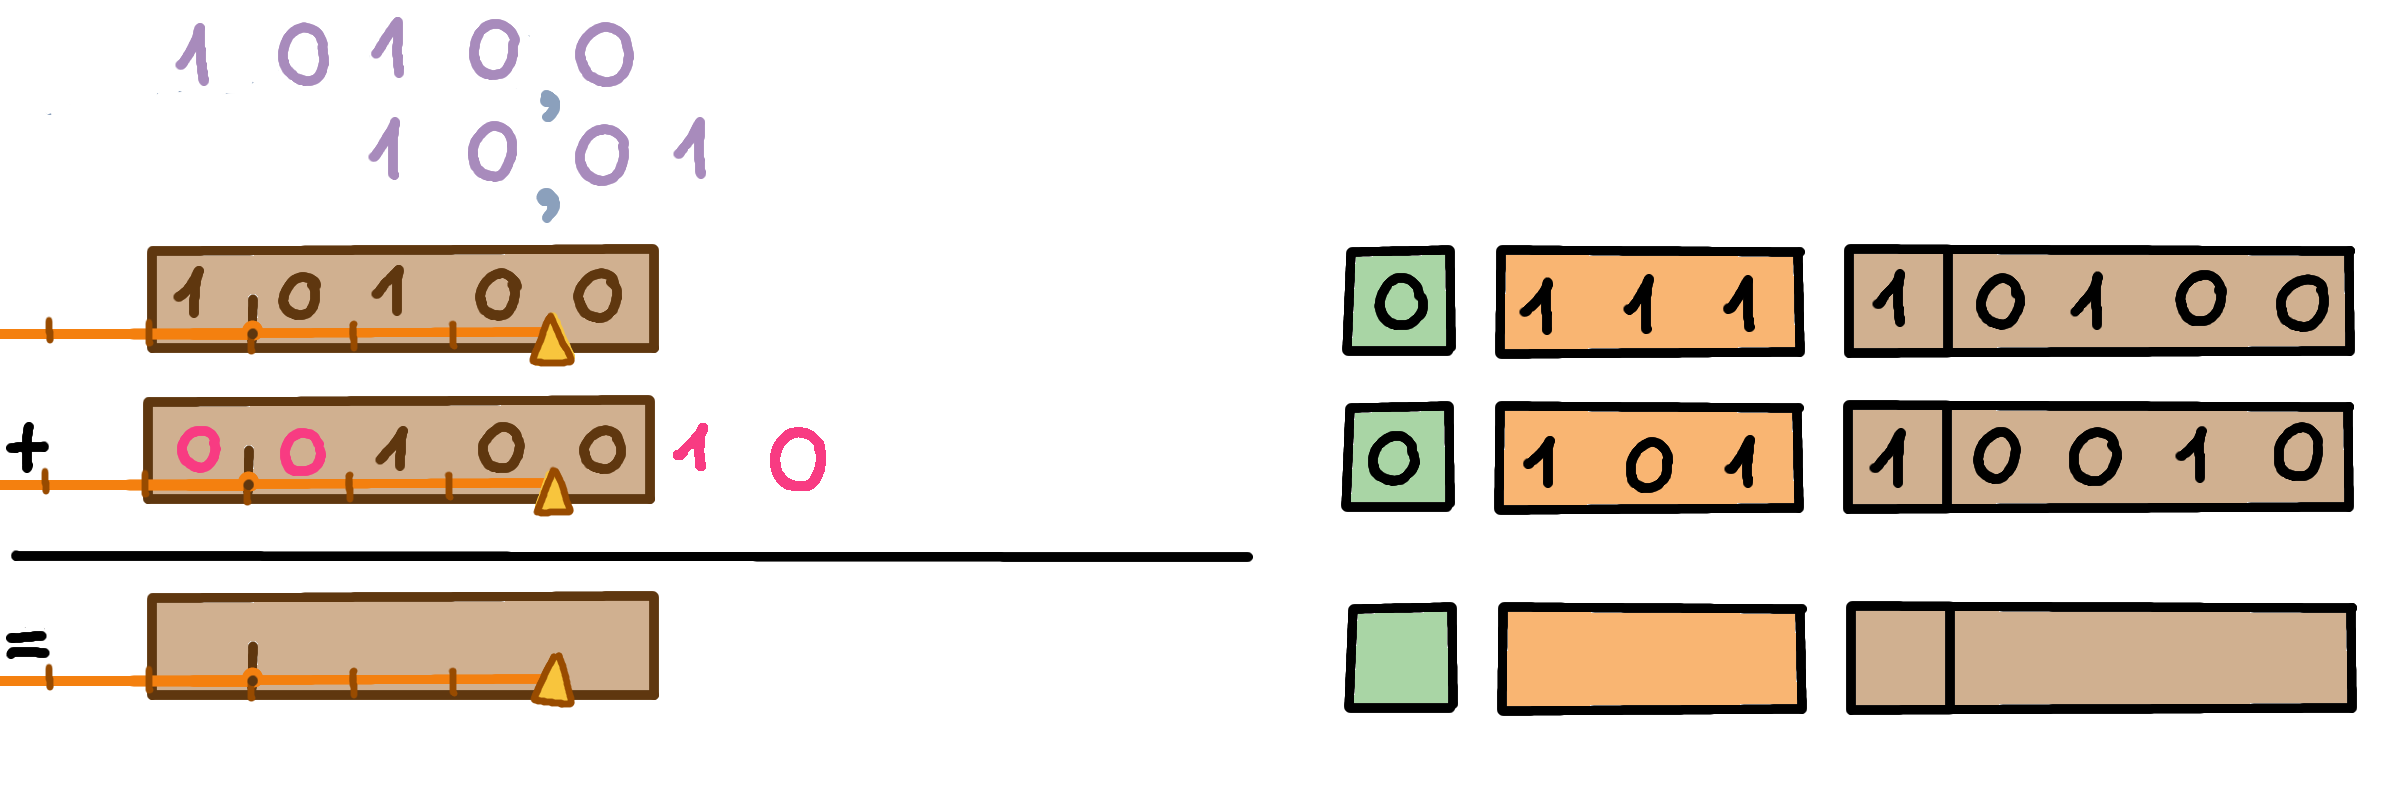
\includegraphics[width=\linewidth]{Pictures/Addition10and2-25_2.png}
\end{figure}

Nun können wir die Bits stellenweise zusammenrechnen.
\begin{figure}[H]
\centering
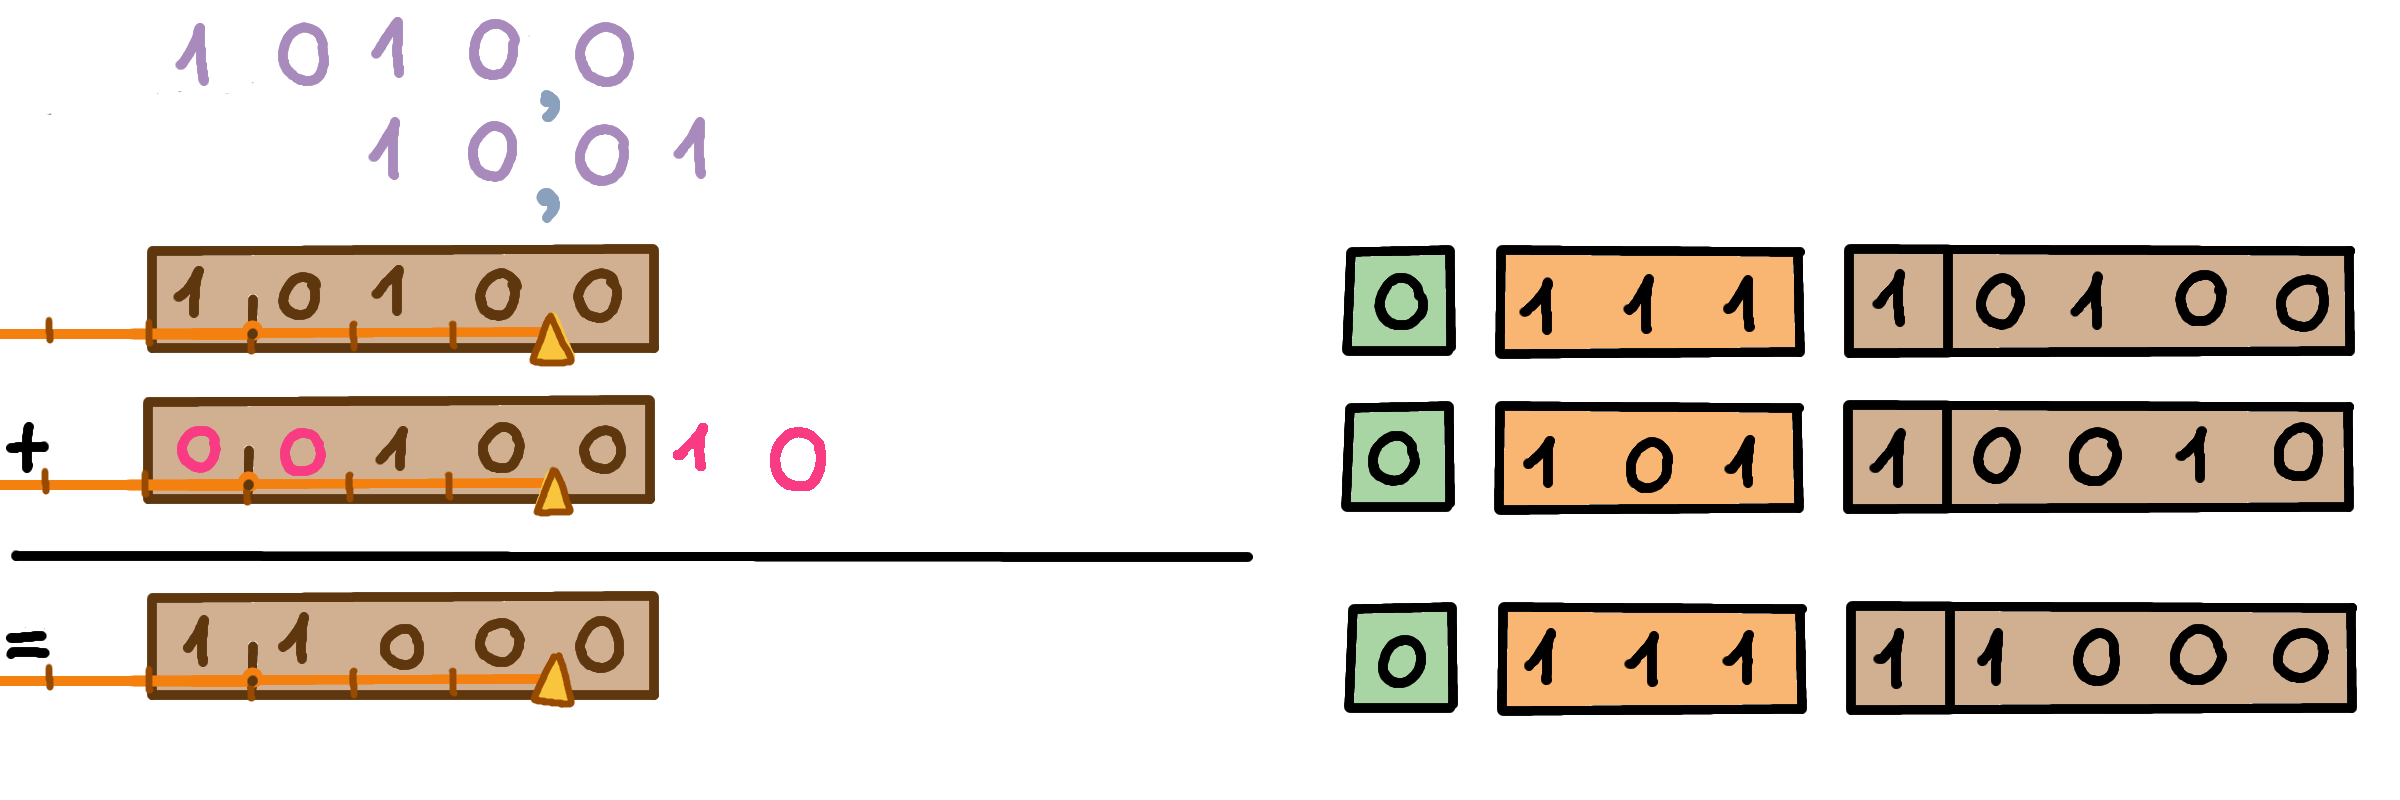
\includegraphics[width=\linewidth]{Pictures/Addition10and2-25_3.png}
\end{figure}

\item \(17/16 + 2 = 3\), in der Exponentialschreibweise \(1.1000 \cdot 2^1\).

Im ersten Schritt schreiben wir die Zahlen auf.
\begin{figure}[H]
\centering
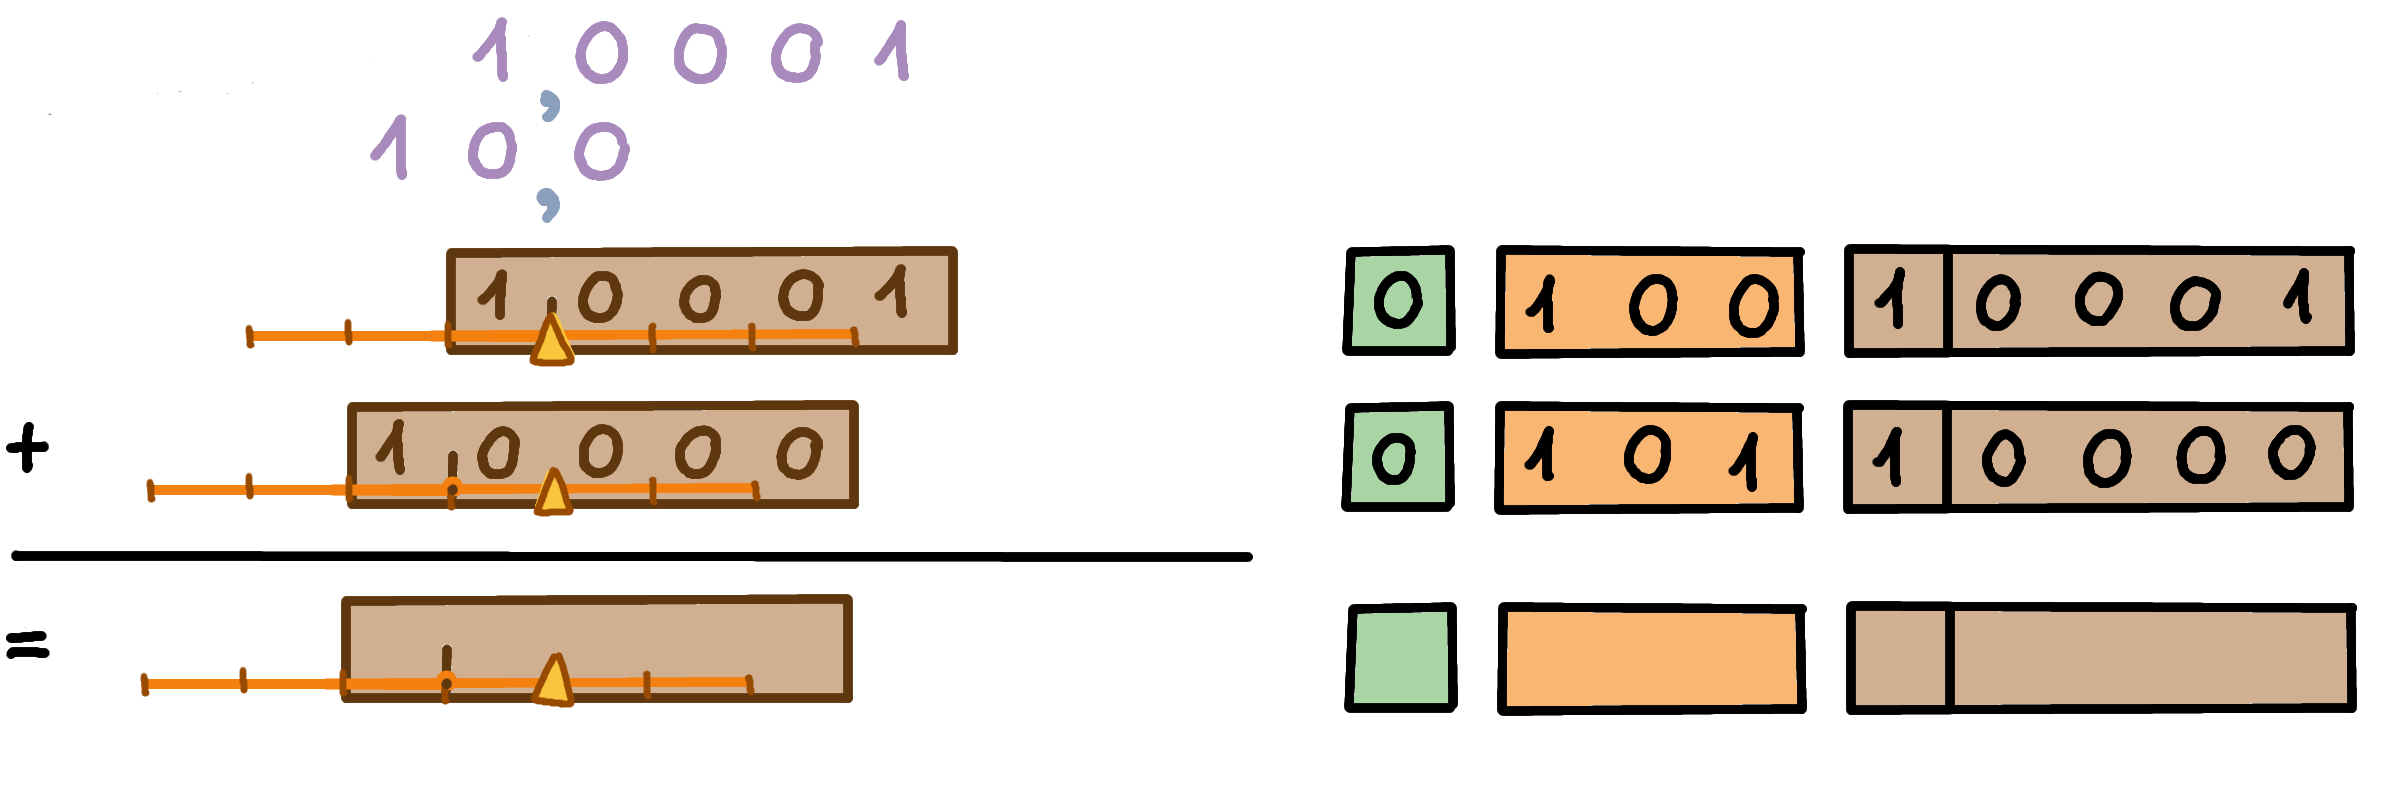
\includegraphics[width=\linewidth]{Pictures/Addition17-16and2_1.png}
\end{figure}

Im zweiten Schritt schiben wir den Kasten von der kleinsten Zahl unter den Kasten der grössten Zahl. Dabei geht eine Stelle verloren.
\begin{figure}[H]
\centering
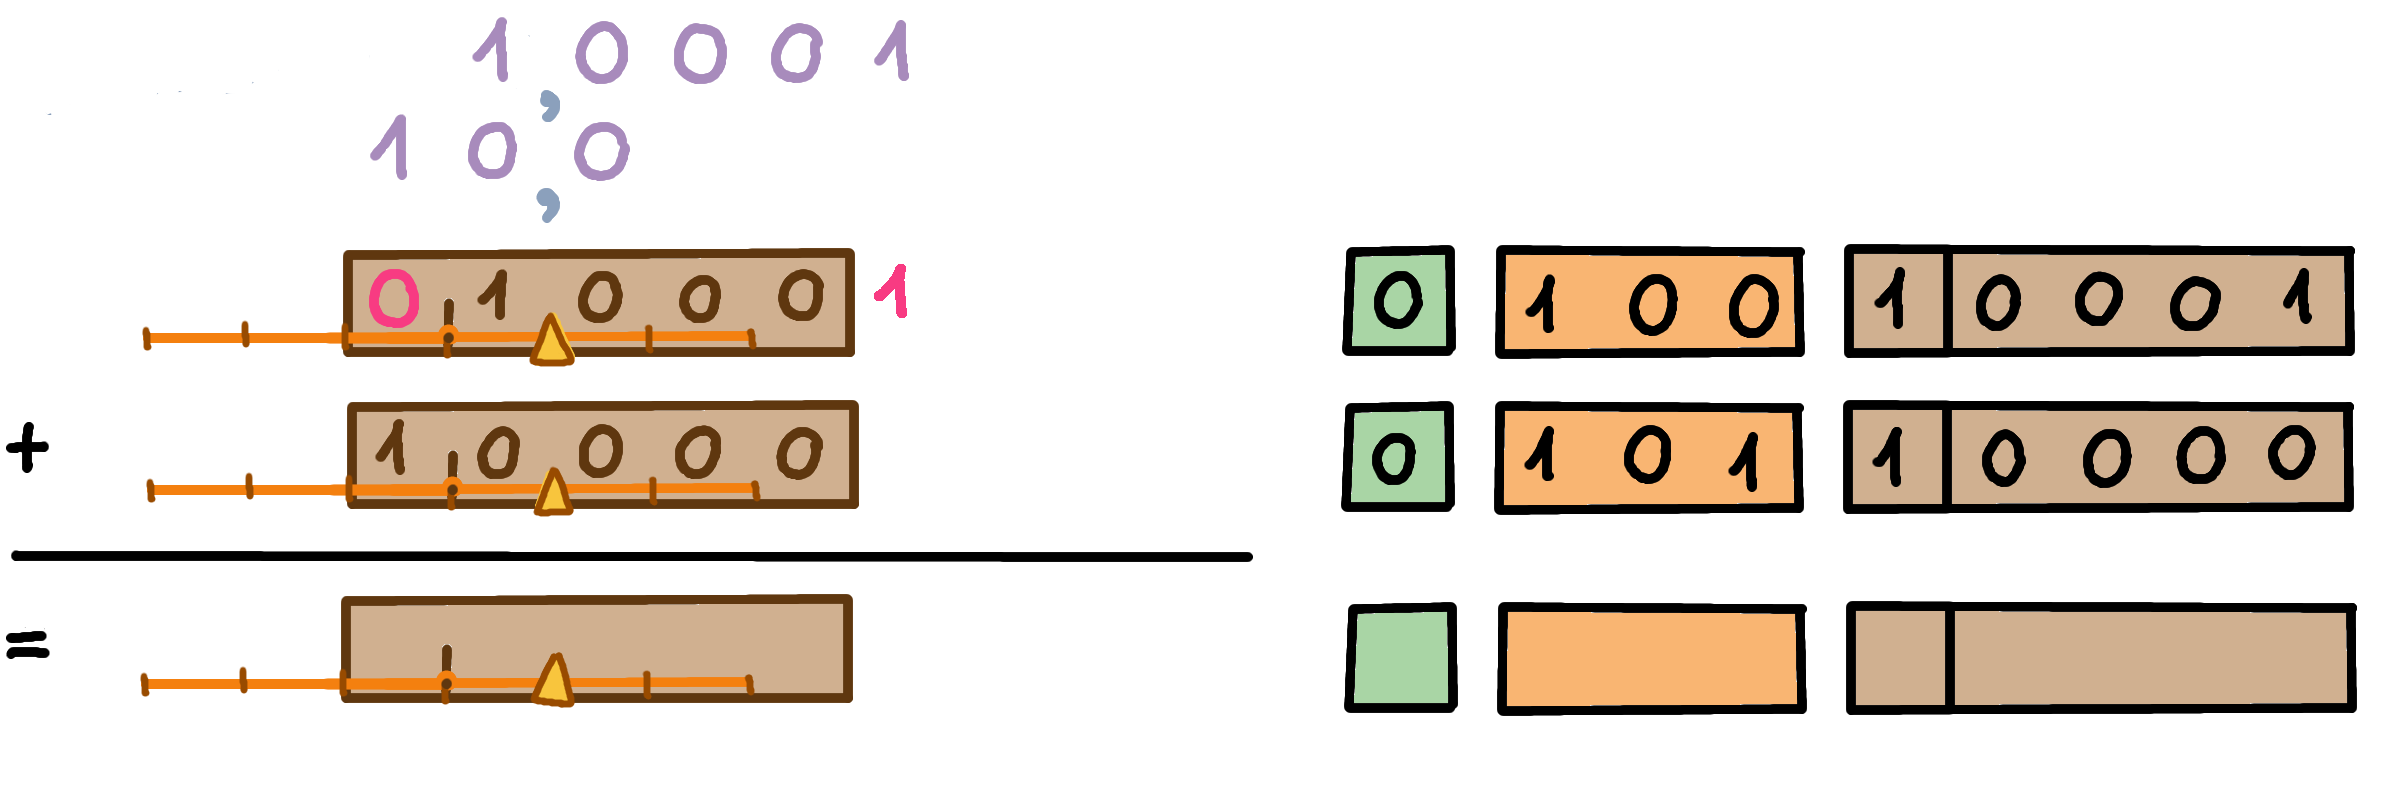
\includegraphics[width=\linewidth]{Pictures/Addition17-16and2_2.png}
\end{figure}

Nun können wir die Bits stellenweise zusammenrechnen.
\begin{figure}[H]
\centering
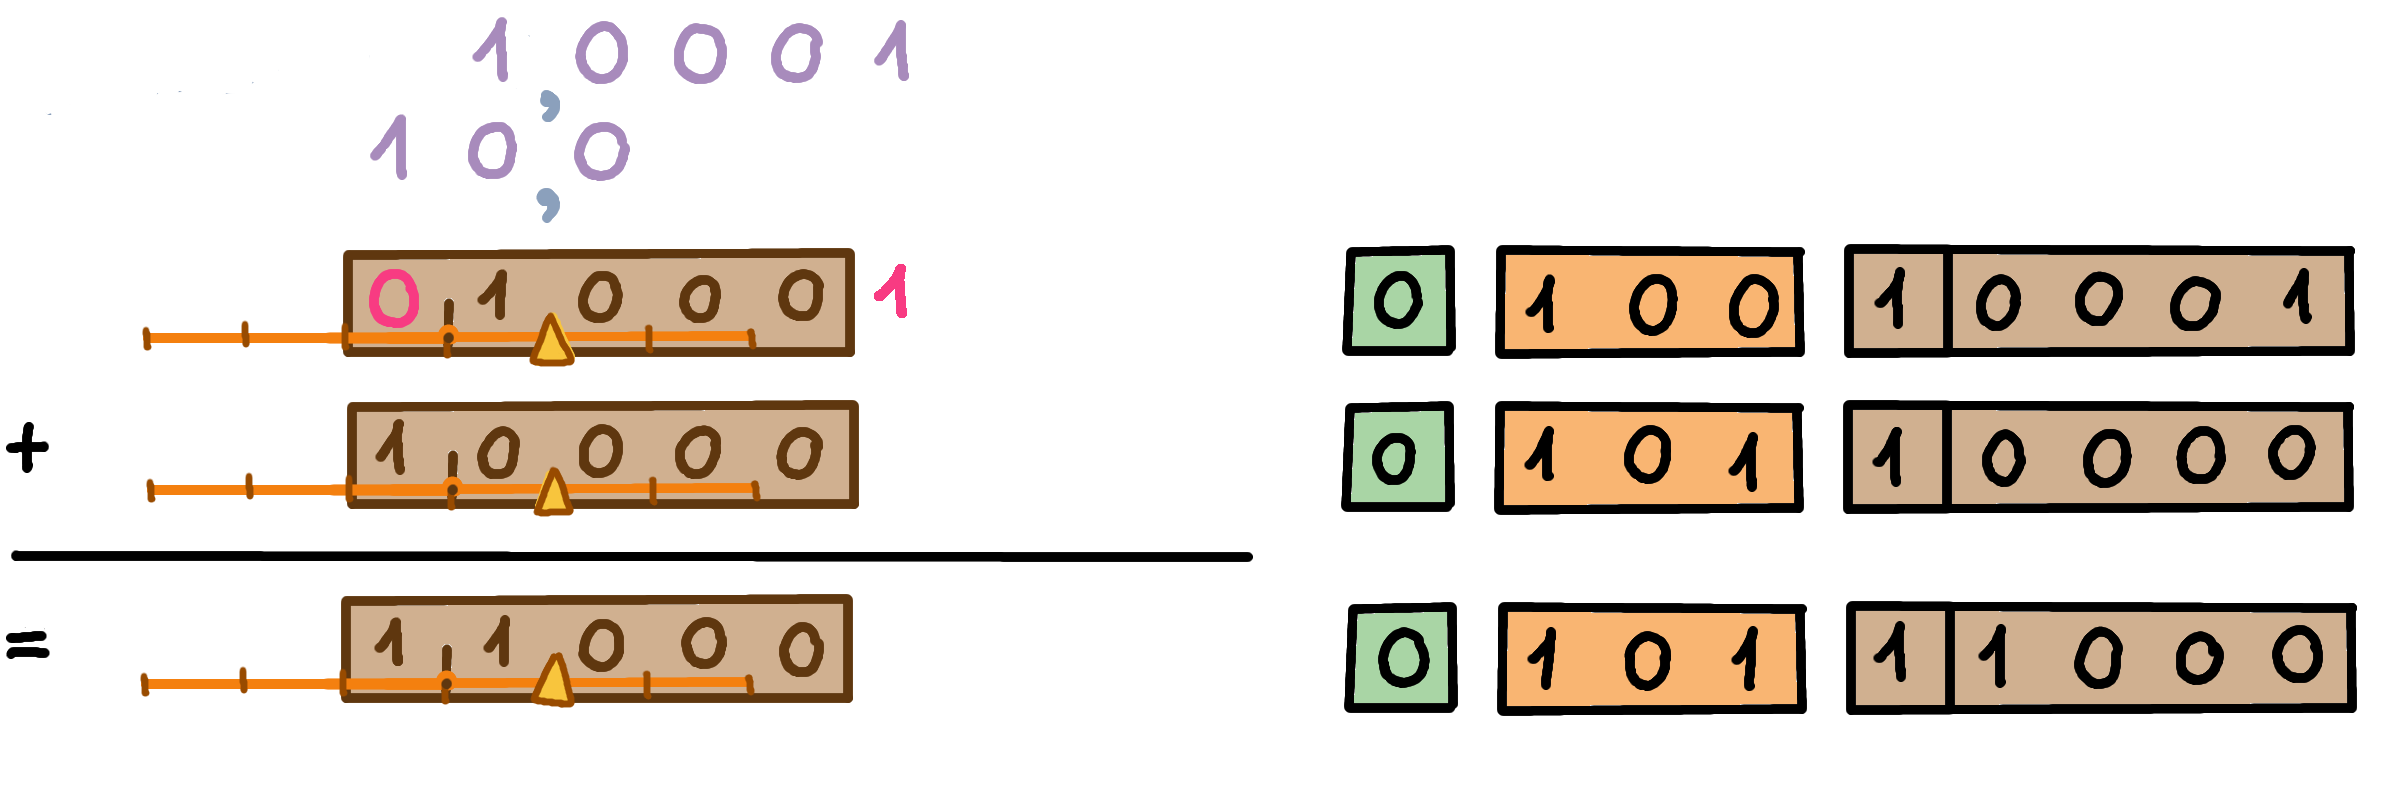
\includegraphics[width=\linewidth]{Pictures/Addition17-16and2_3.png}
\end{figure}

\end{enumerate}

%--------------------------------

\paragraph{Aufgabe \ref{ein_achtel}} Die maximale Zahl, die wir erreichen können, wenn wir \(1/8 + 1/8 + \dotsb + 1/8\) zusammen rechnen, ist \(4.0\).

Zum einen, wenn wir die \(4.0\) erreicht haben, kommen wir nicht mehr weiter.
Das sehen wir, wenn wir \(4.0 + 1/8\) ausrechnen. Wie gewöhnlich schreiben wir zuerst die Summanden untereinander.
\begin{figure}[H]
\centering
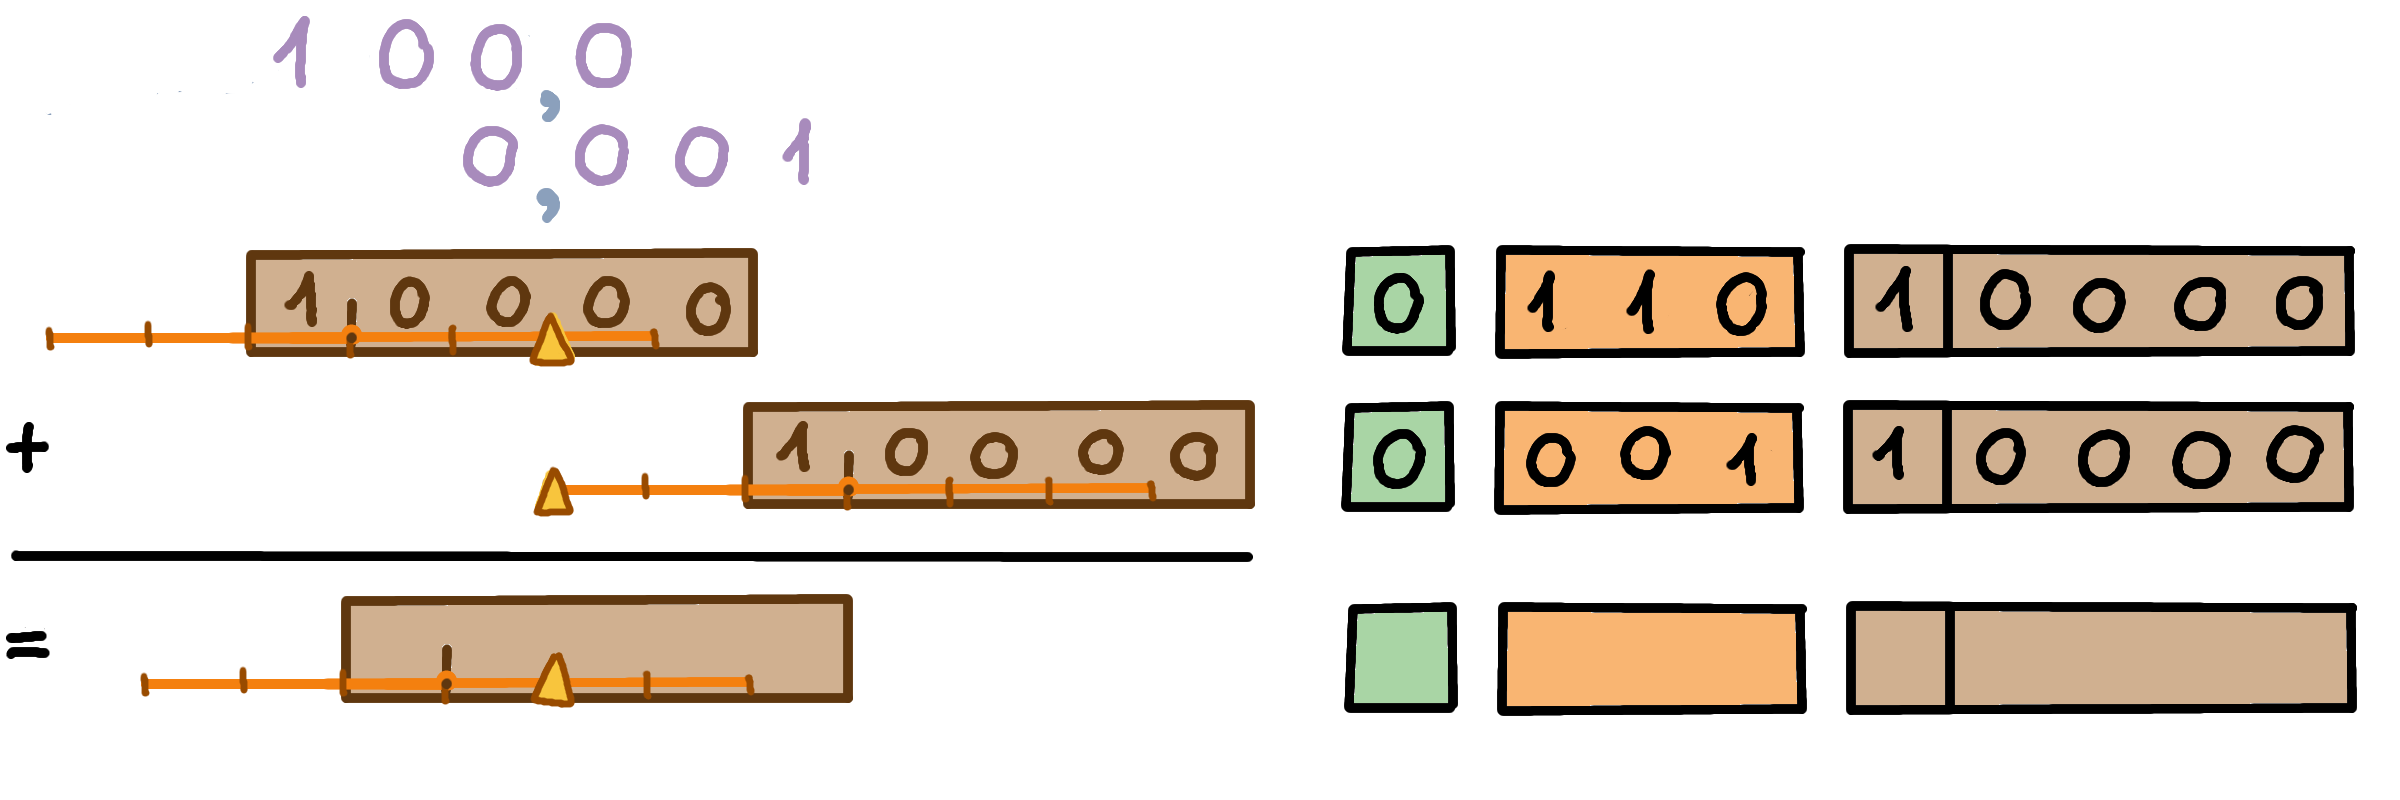
\includegraphics[width=\linewidth]{Pictures/Addition4and1-8_1.png}
\end{figure}
Wenn wir den Kasten von \(1/8\) unter den Kasten von \(4.0\) verschieben, sehen wir, dass alle signifikanten Stellen von \(1/8\) verloren gehen, auch die führende Eins.
\begin{figure}[H]
\centering
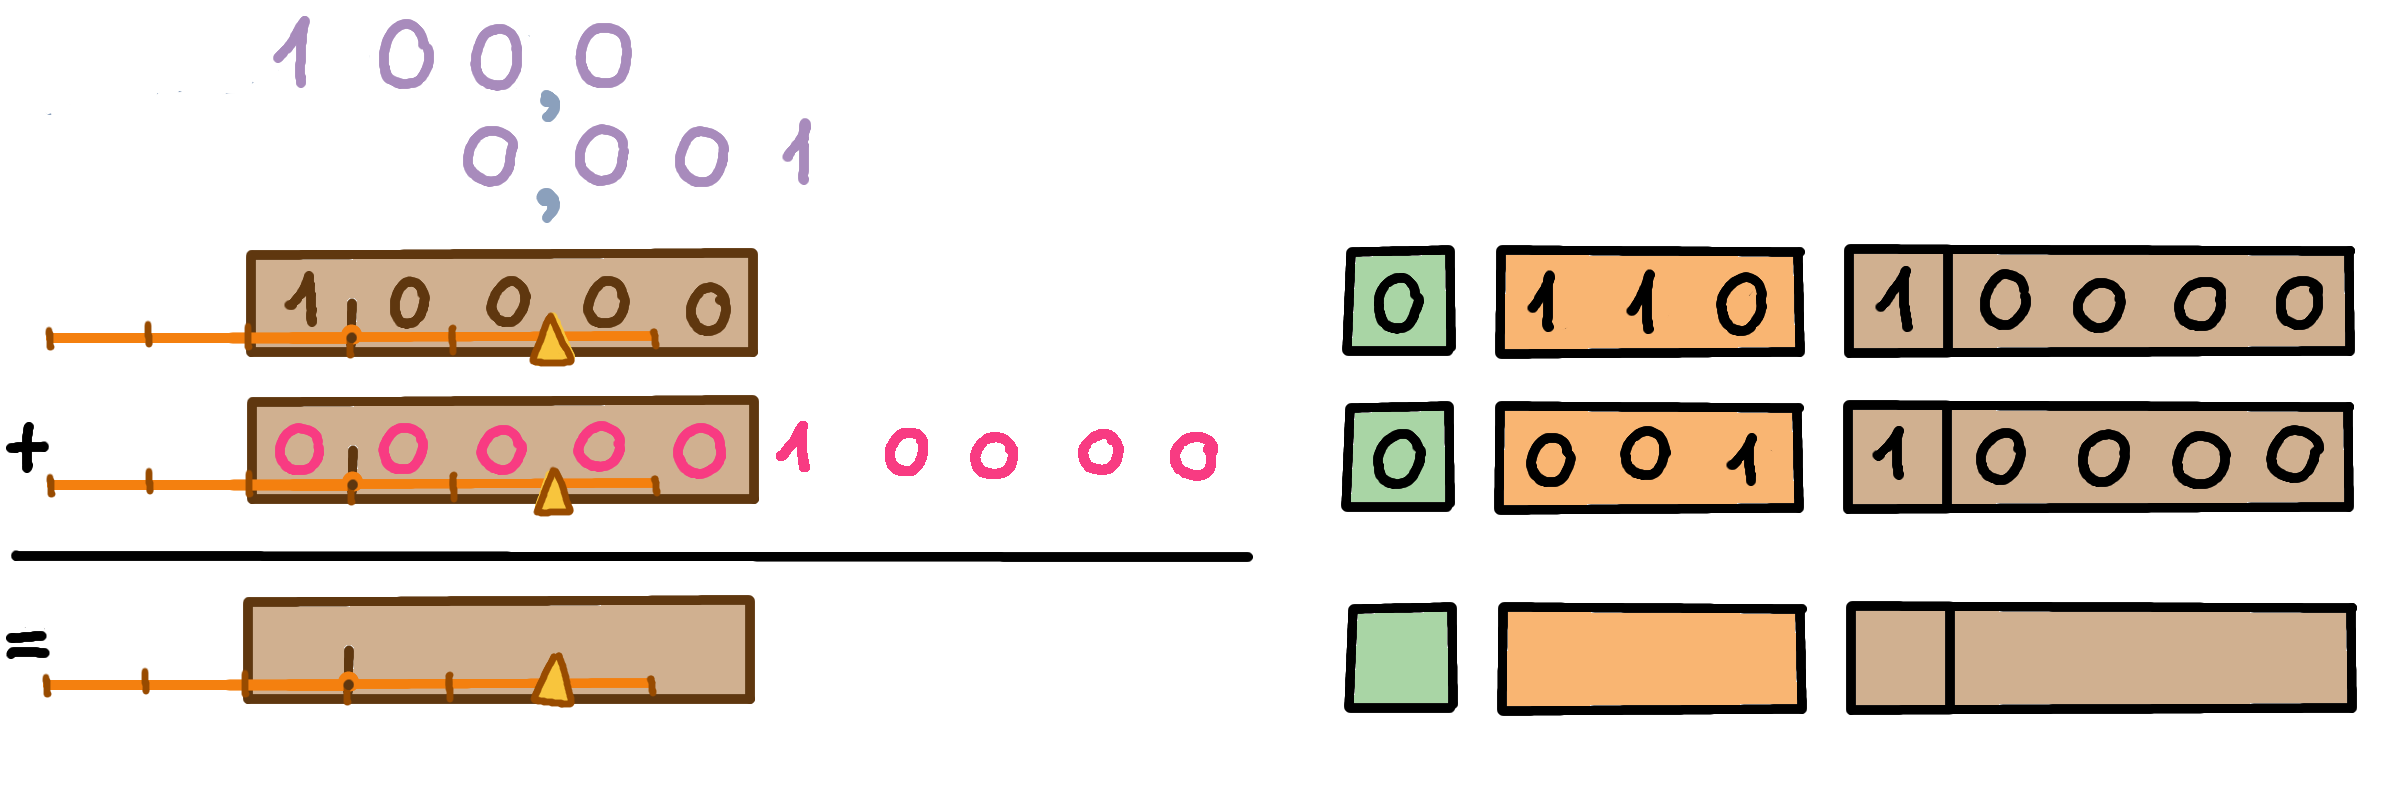
\includegraphics[width=\linewidth]{Pictures/Addition4and1-8_2.png}
\end{figure}
Deswegen, wenn wir \(4.0 + 1/8\) ausrechnen, kriegen wir \(4.0\).
\begin{figure}[H] 
\centering
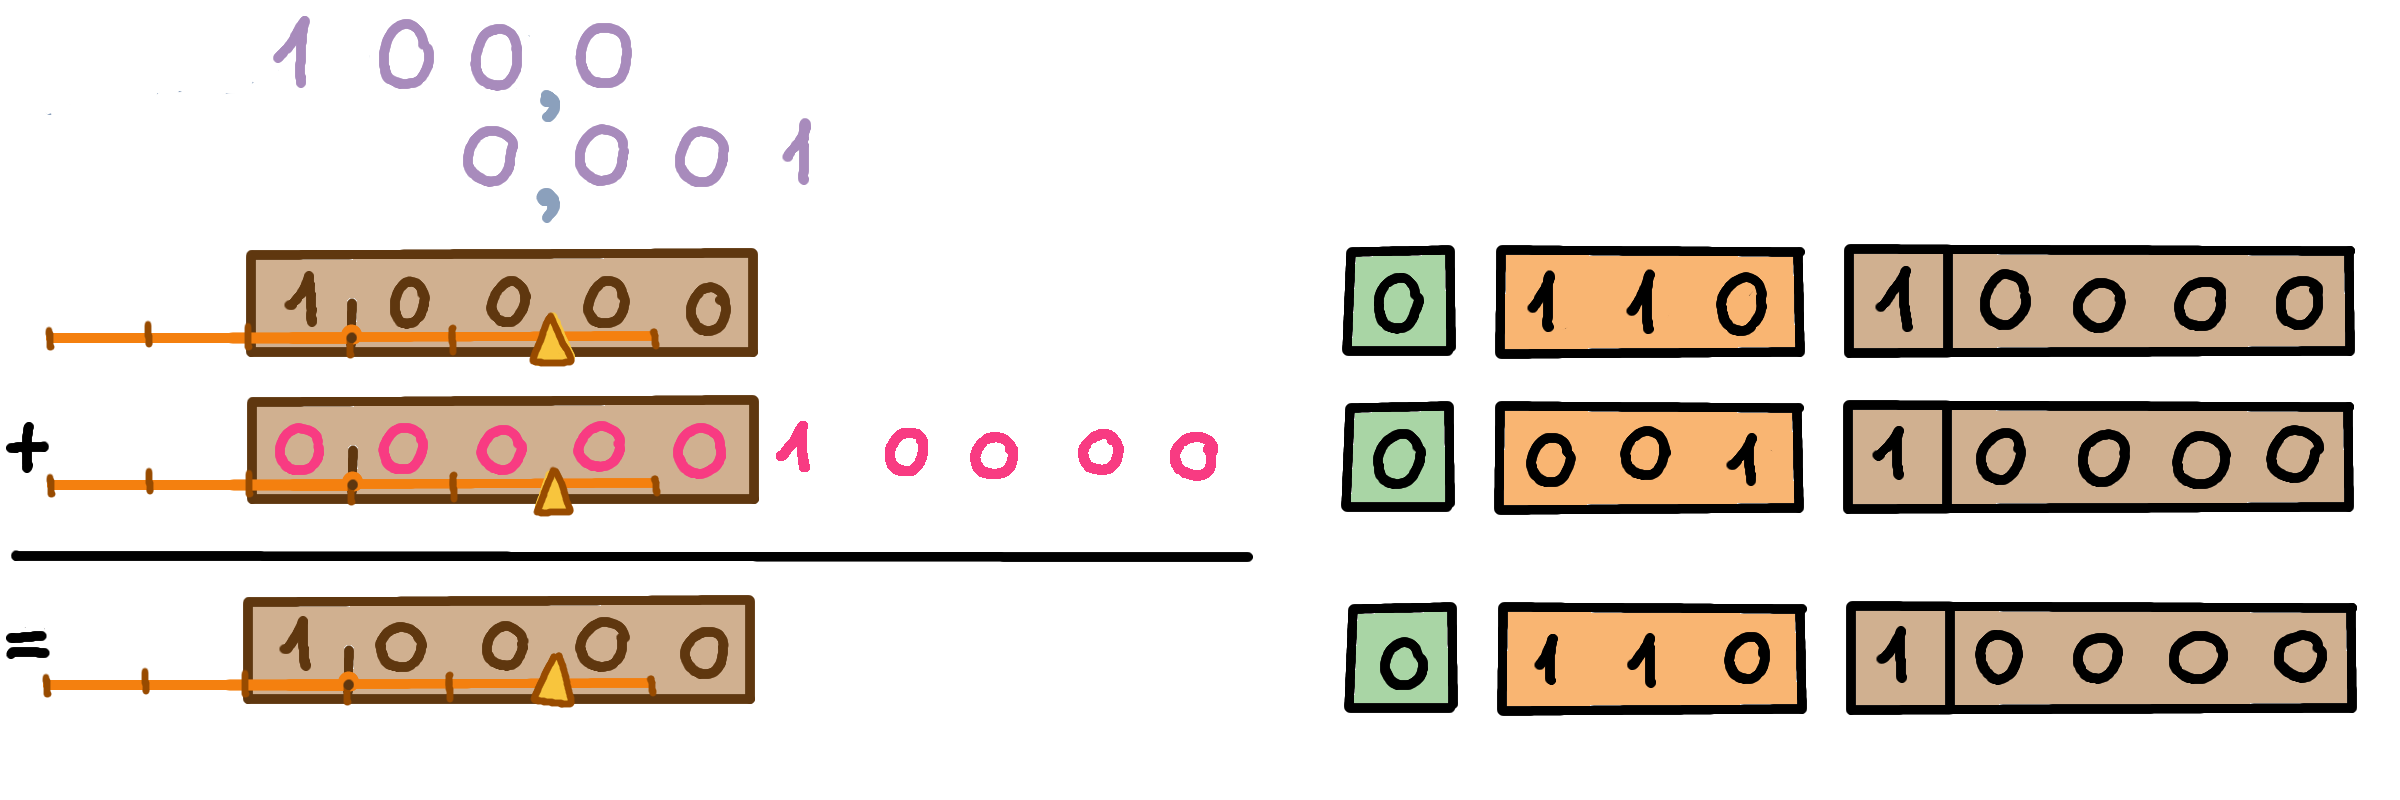
\includegraphics[width=\linewidth]{Pictures/Addition4and1-8_3.png} 
\end{figure}
Egal wie viele \(1/8\) rechnen wir zusammen, bleiben wir immer bei \(4.0\).

Jetzt bleibt uns zu zeigen, dass wir die \(4.0\) auch tatsächlich erreichen können. Das Problem bei der \(4.0\) ist, dass alle signifikanten Stellen von \(1/8\) verloren gehen. Das passiert, weil der Unterschied zwischen dem Exponenten von \(4.0\) und dem Exponenten von \(1/8\) die ganze Mantissenlänge beträgt. Das passiert bei einem kleineren Exponenten nicht. Zum Beispiel, wenn wir \(2.0 + 1/8\) ausrechnen, sehen wir, dass das Ergebnis wie erwartet \(17/8\) ist.

Um zu zeigen, dass das Problem erst bei \(4.0 + 1/8\) auftritt, rechnen wir \(2.0 + 1/8\). Das Ergebnis ist wie erwartet \(17/8\).
\begin{figure}[H]
\centering
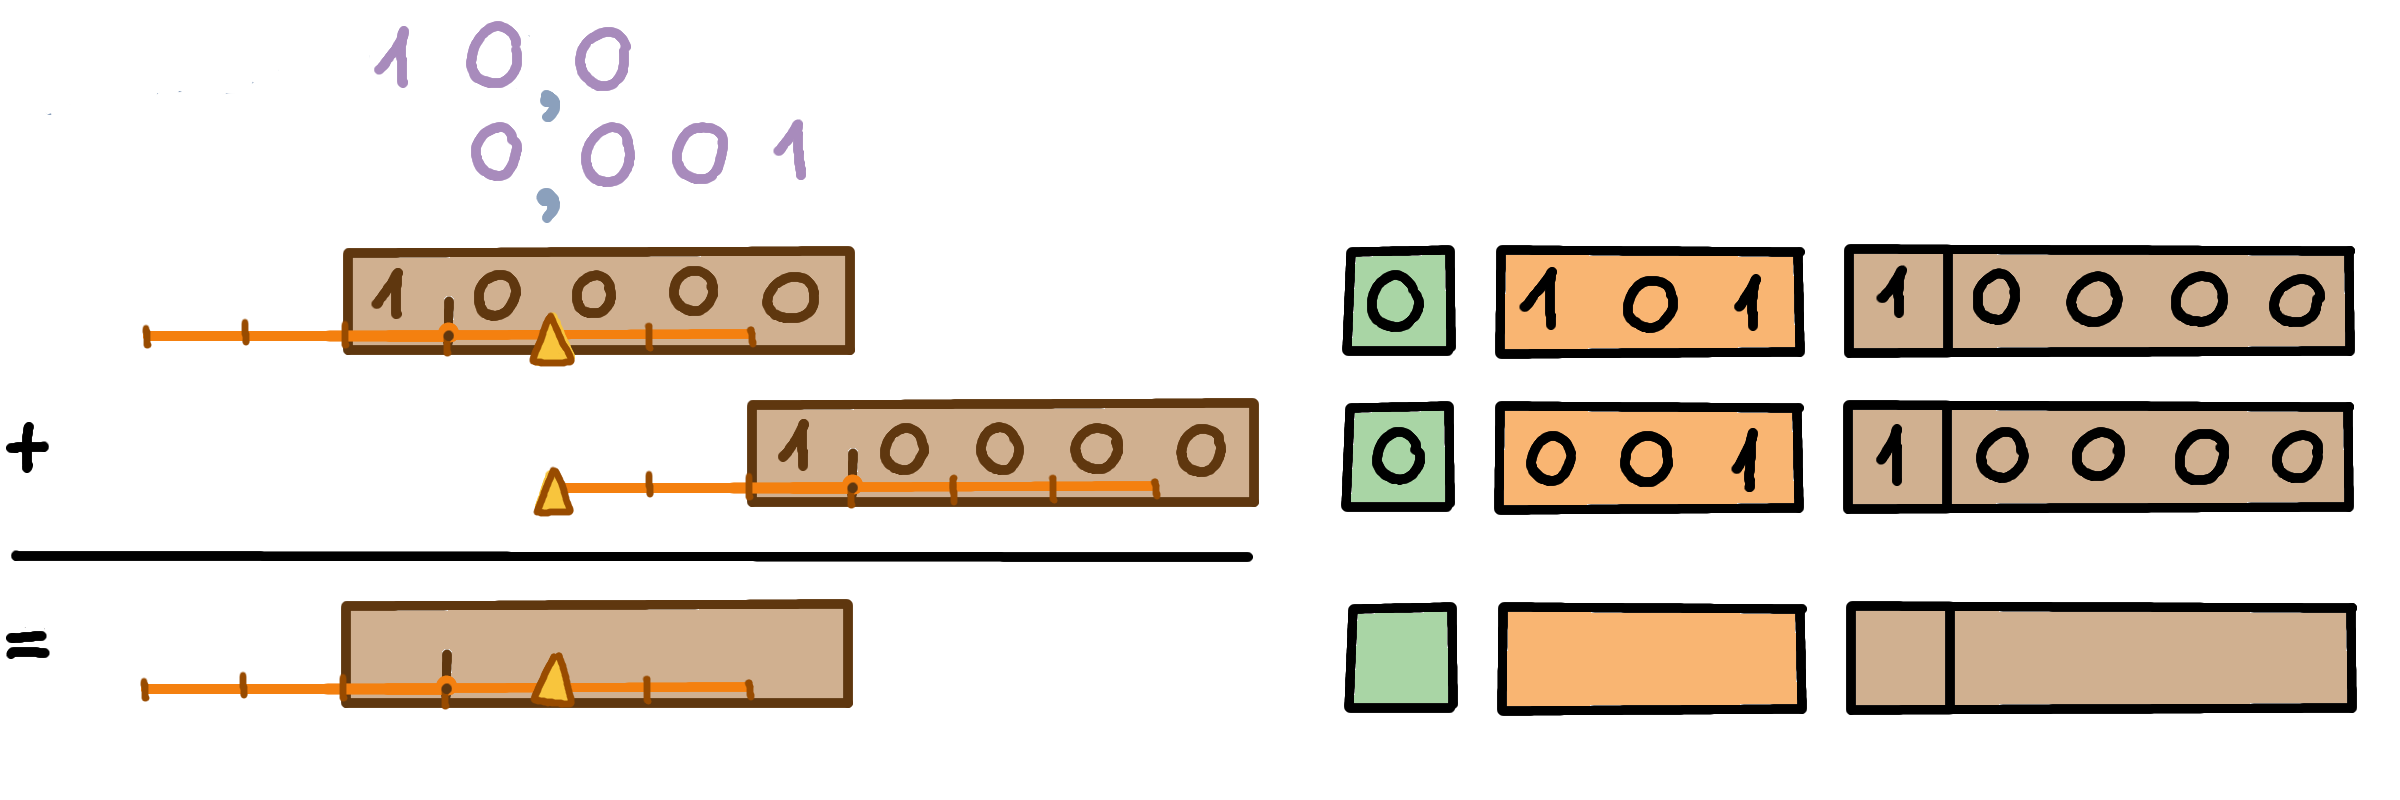
\includegraphics[width=\linewidth]{Pictures/Addition2and1-8_1.png} 
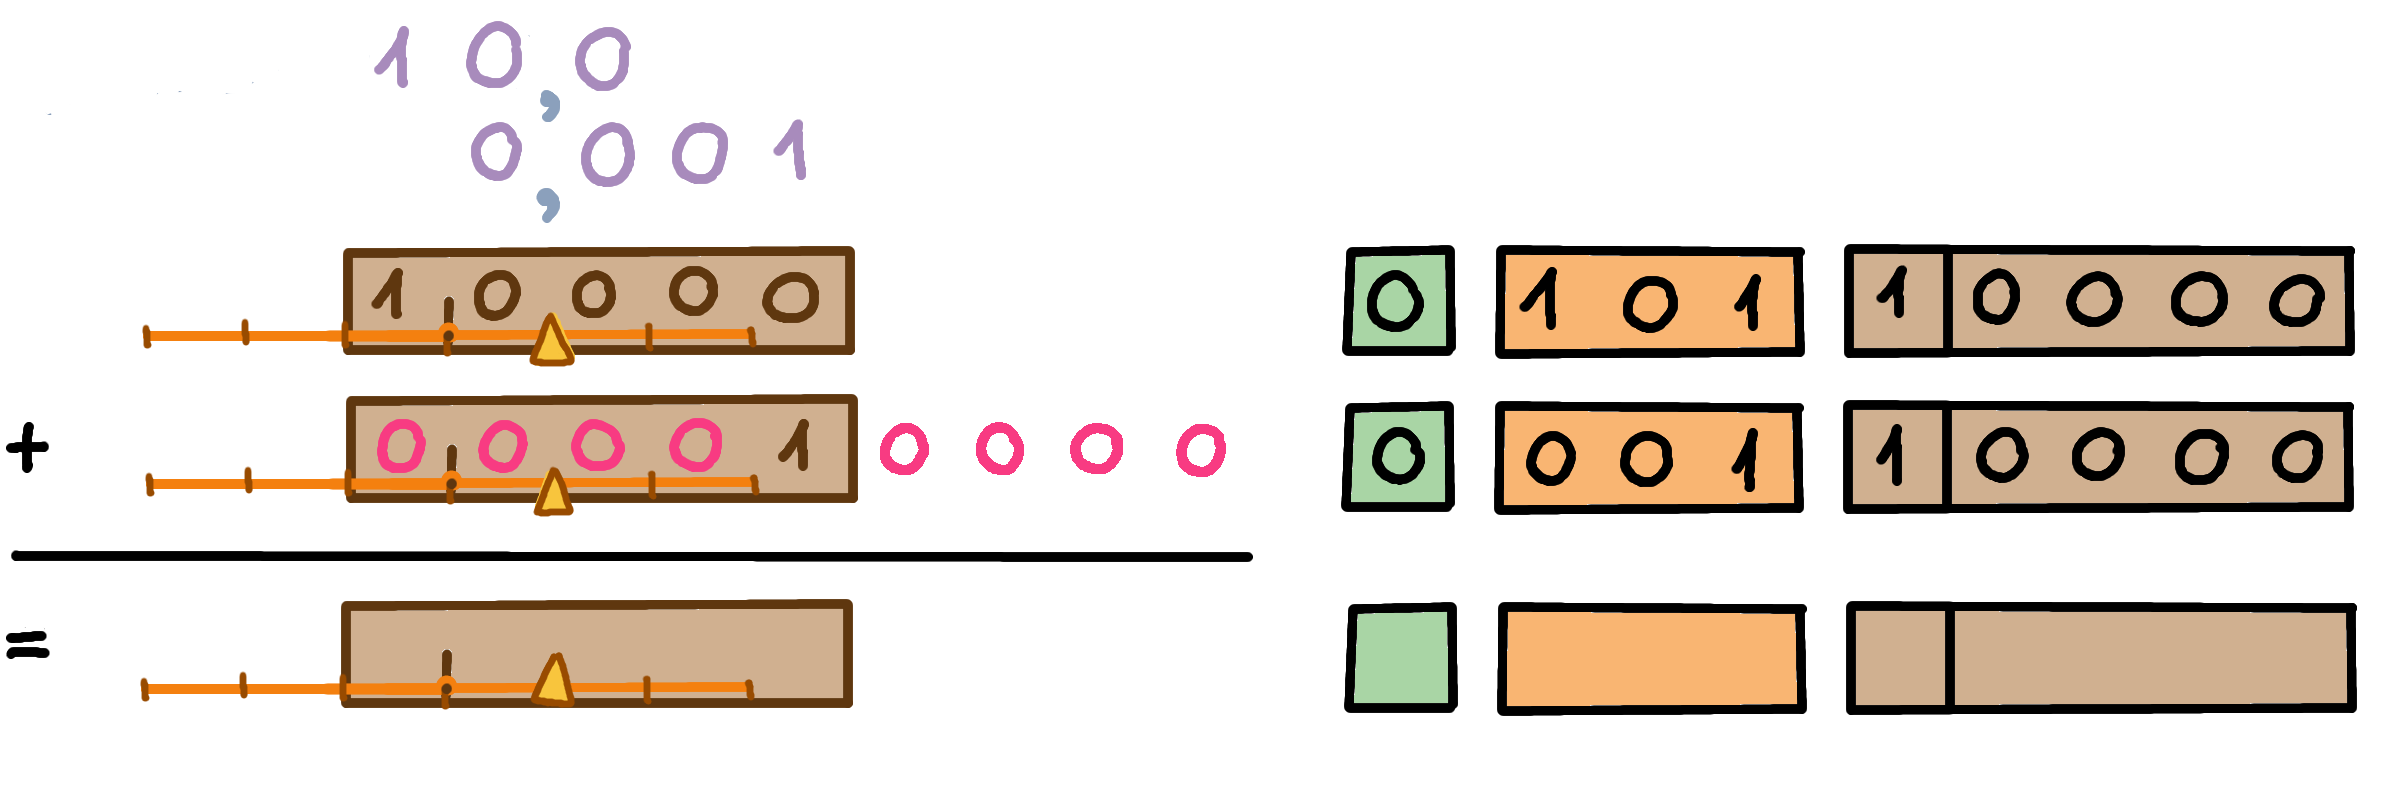
\includegraphics[width=\linewidth]{Pictures/Addition2and1-8_2.png} 
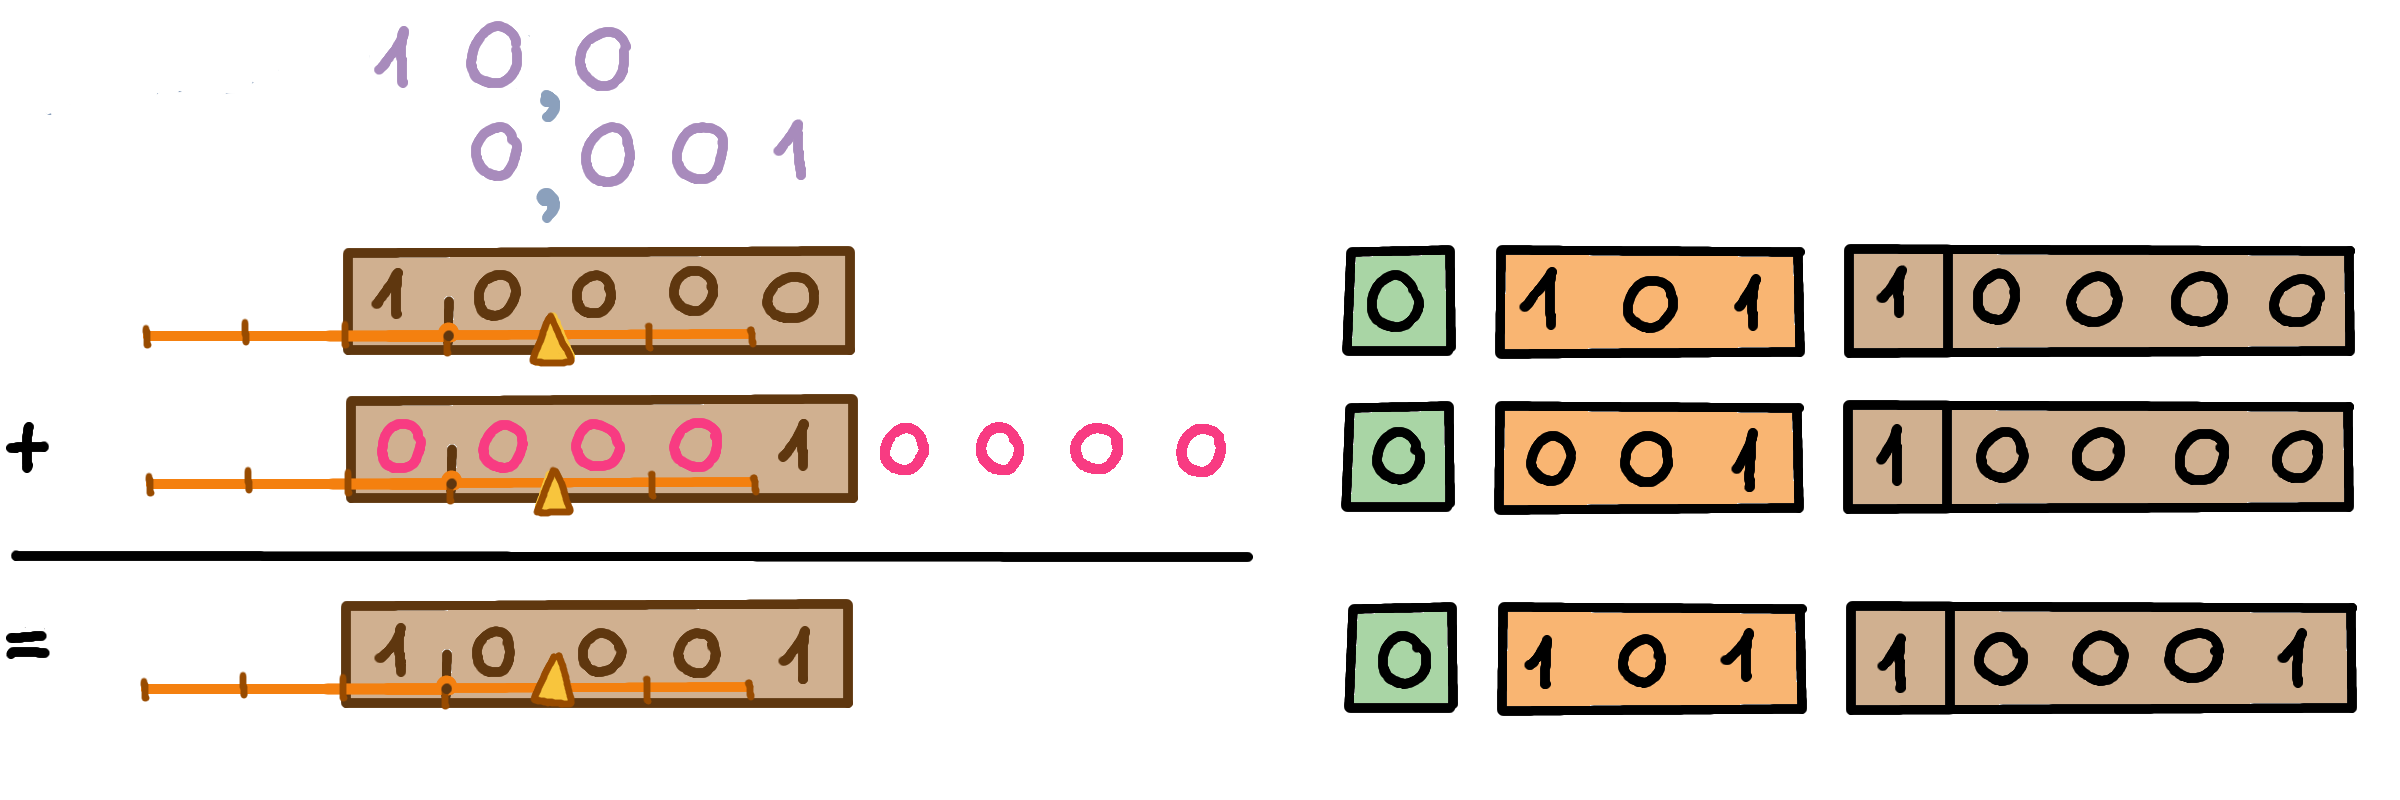
\includegraphics[width=\linewidth]{Pictures/Addition2and1-8_3.png} 
\end{figure}
Wir erreichen also die \(4.0\) nach 32 Summanden und kommen dann nicht mehr weiter.

%--------------------------------

\paragraph{Aufgabe \ref{addition_kontrollfragen}}
\begin{enumerate}[(a)]
\item Der Wert der Bits in der Mantisse hängt vom Exponenten ab. Zum Beispiel, dieselbe Mantisse \(1.0000\) mit unterschiedlichen Exponenten kann \(4\), \(2\), \(1\), \(1/2\), \(1/4\) und \(1/8\) darstellen. Wir wollen nicht, dass \(1+2\) das gleiche Ergebnis liefert die \(1 + 1/4\). Wir wollen nur Bits mit dem gleichen Wert zusammen addieren. Deswegen müssen wir vor der Addition sicherstellen, dass die Kasten der beiden Summanden exakt untereinander stehen.

\item Die Aussage von Gregory ist falsch. Der Kasten vom Ergebnis kann sich bewegen bezüglich des Kastens vom grössten Summanden. Dies passiert, zum Beispiel, wenn man \(2.5 + 1.75\) ausrechnet.

\item Hannah hat teilweise recht. Die Addition bei den Fliesskommazahlen ist kommutativ aber nicht assoziativ.

Wenn wir zwei Zahlen zusammen addieren und diese zwei Zahlen vertauschen, kriegen wir das gleiche Ergebnis auch bei Fliesskommazahlen.

Wenn wir aber die Reihenfolge verändern, in welcher die Zahlen zusammengerechnet werden, können wir unterschiedlich Ergebnisse bekommen. Das passiert, weil wir nur dann den exakten Wert ausrechnen können, wenn die Grössenordnung der Teilsummanden ähnlich ist.
\end{enumerate}

%--------------------------------

\paragraph{Aufgabe \ref{ameisenkönigin}}

Nein, das Programm der Ameisenkönigin wird unendlich lange laufen und die Anzahl Ameisen, die es braucht, um 10 Reiskörnchen zu transportieren, nie ausgeben. Das Problem ist analog zu dem, was wir in Aufgabe \ref{ein_achtel} gesehen haben. Das Programm läuft wie erwartet bis wir die \(8.0\) erreichen. Wenn wir aber \(1/4\) dazu rechnen, dann verlieren wir alle signifikanten Stellen von \(1/4\) und die \(8.0\) bleibt unverändert.
\begin{figure}[H]
\centering
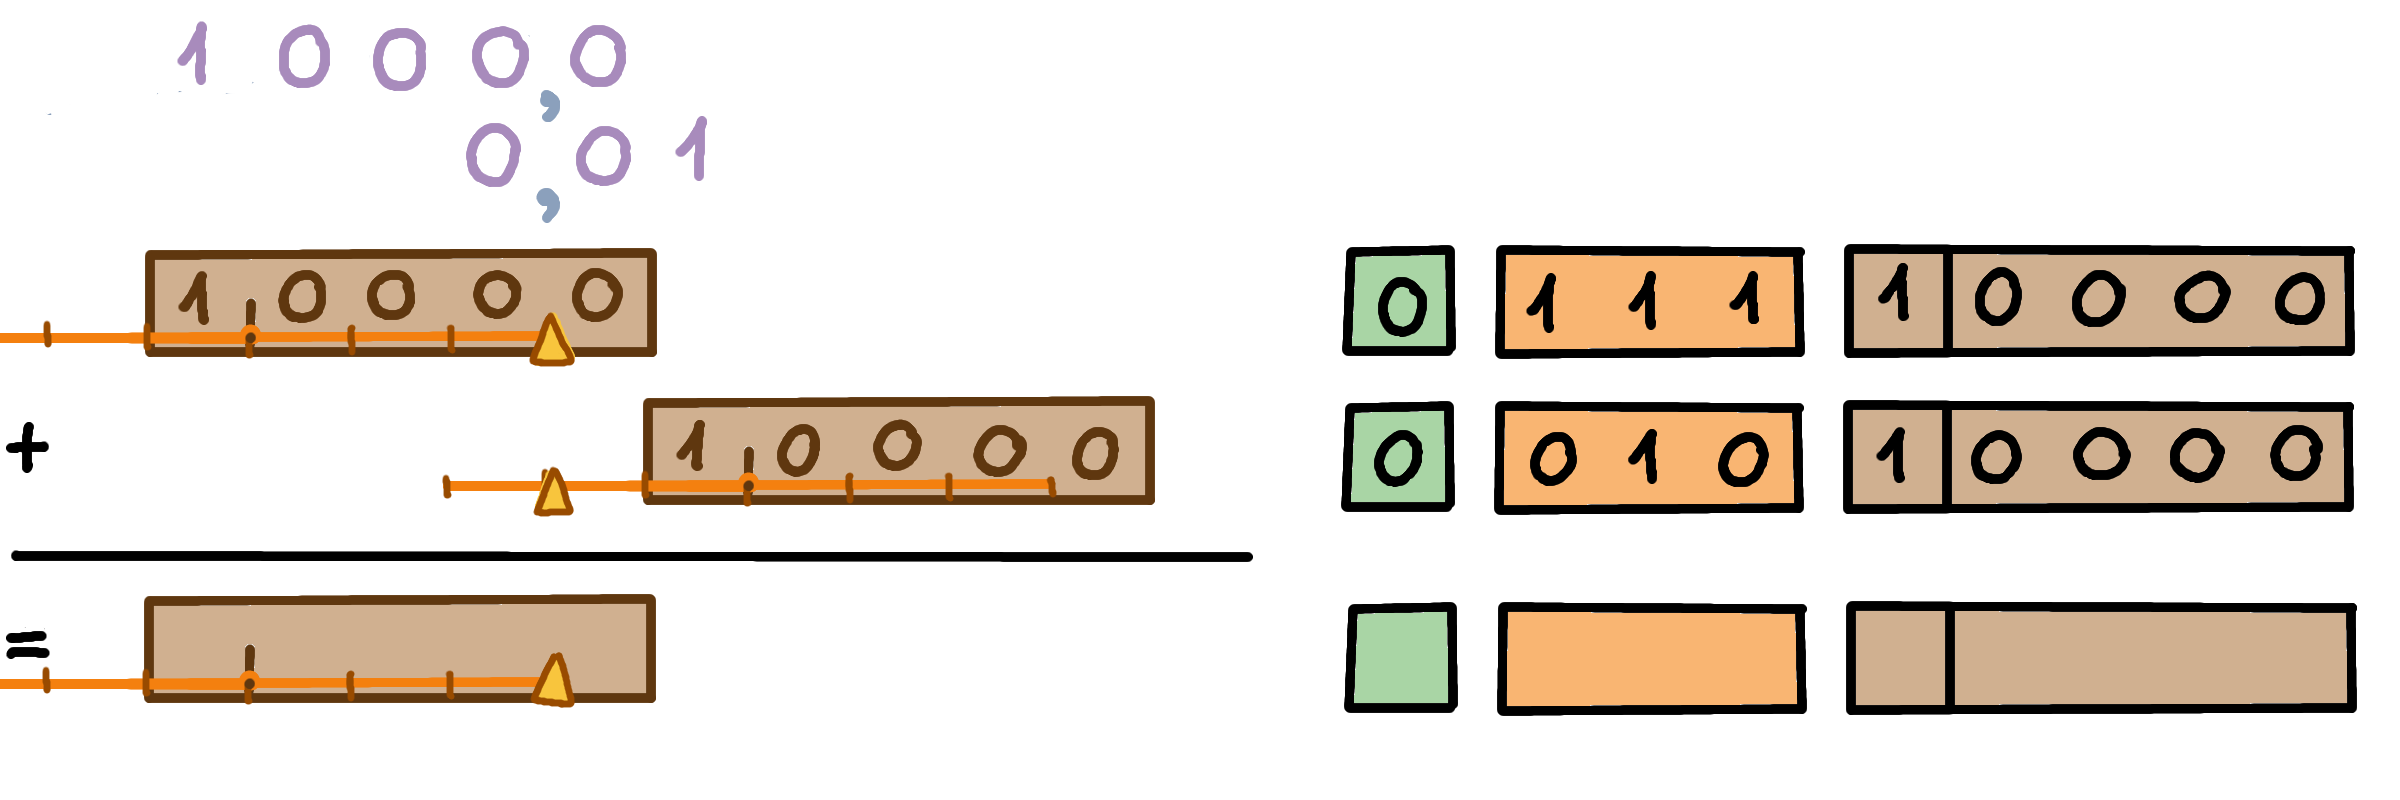
\includegraphics[width=\linewidth]{Pictures/Addition8and1-4_1.png} 
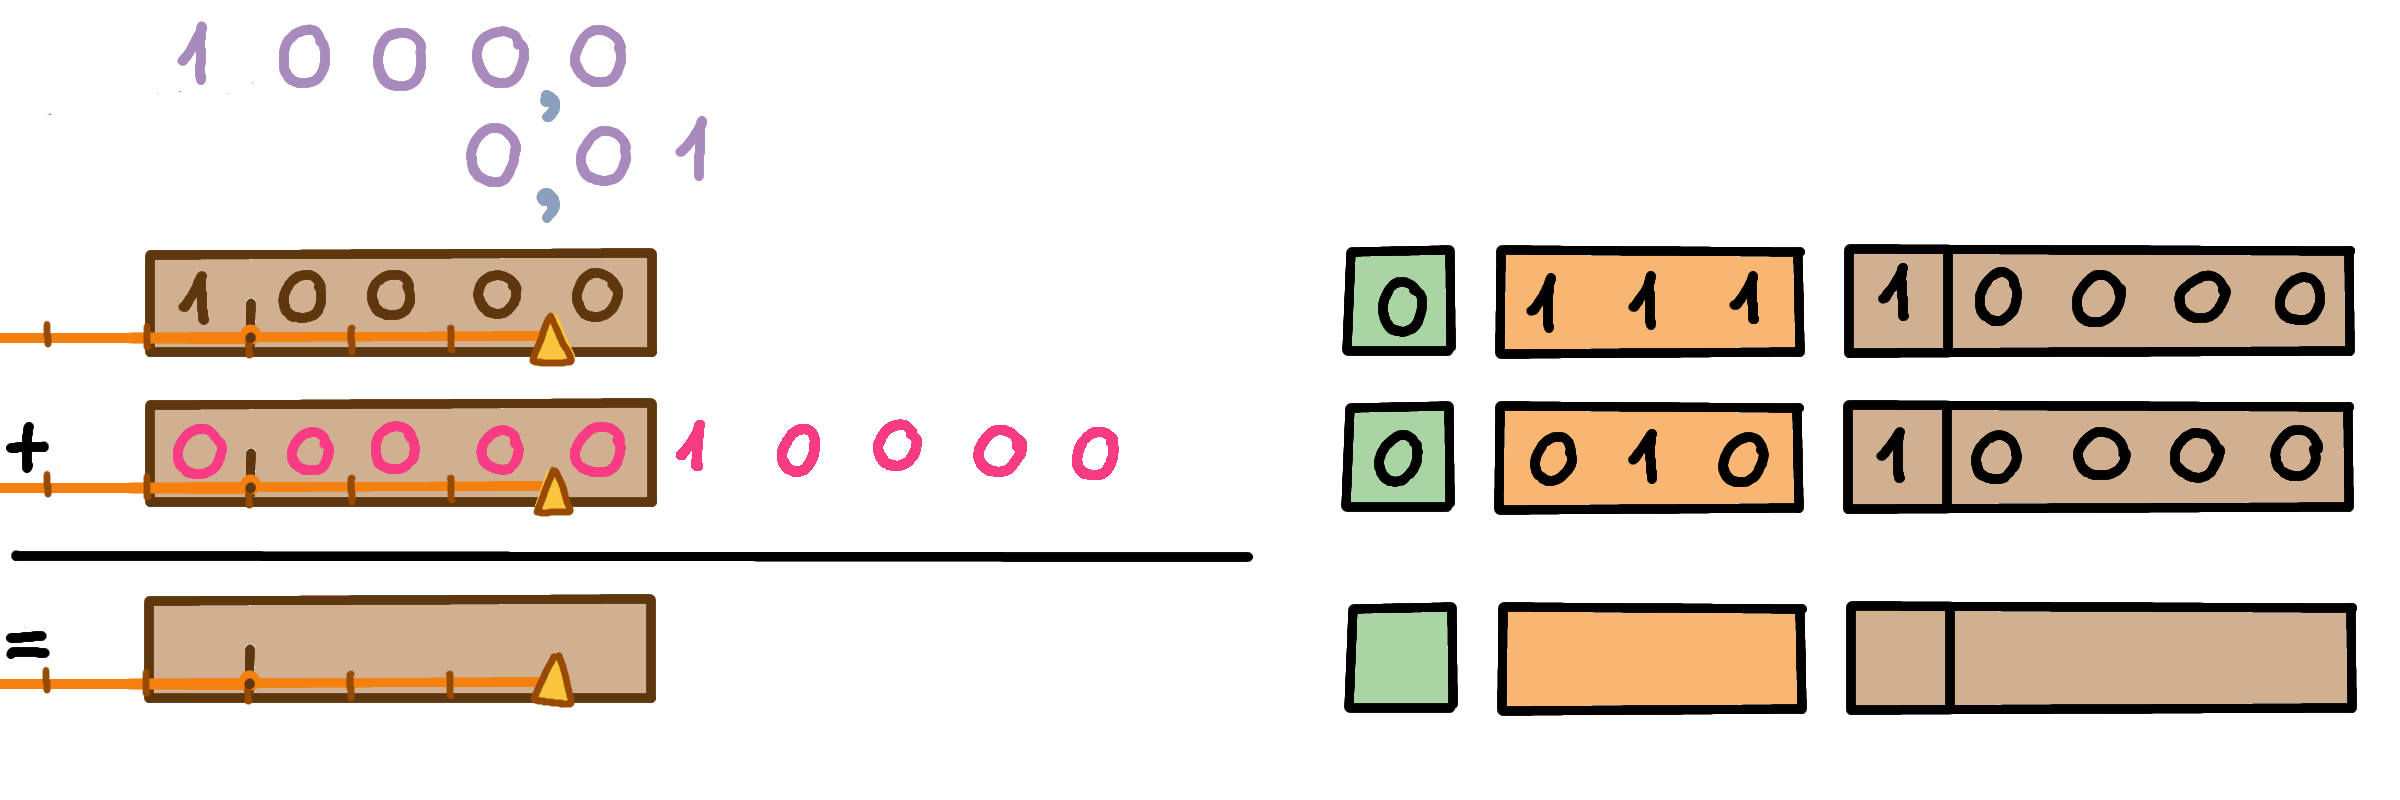
\includegraphics[width=\linewidth]{Pictures/Addition8and1-4_2.png} 
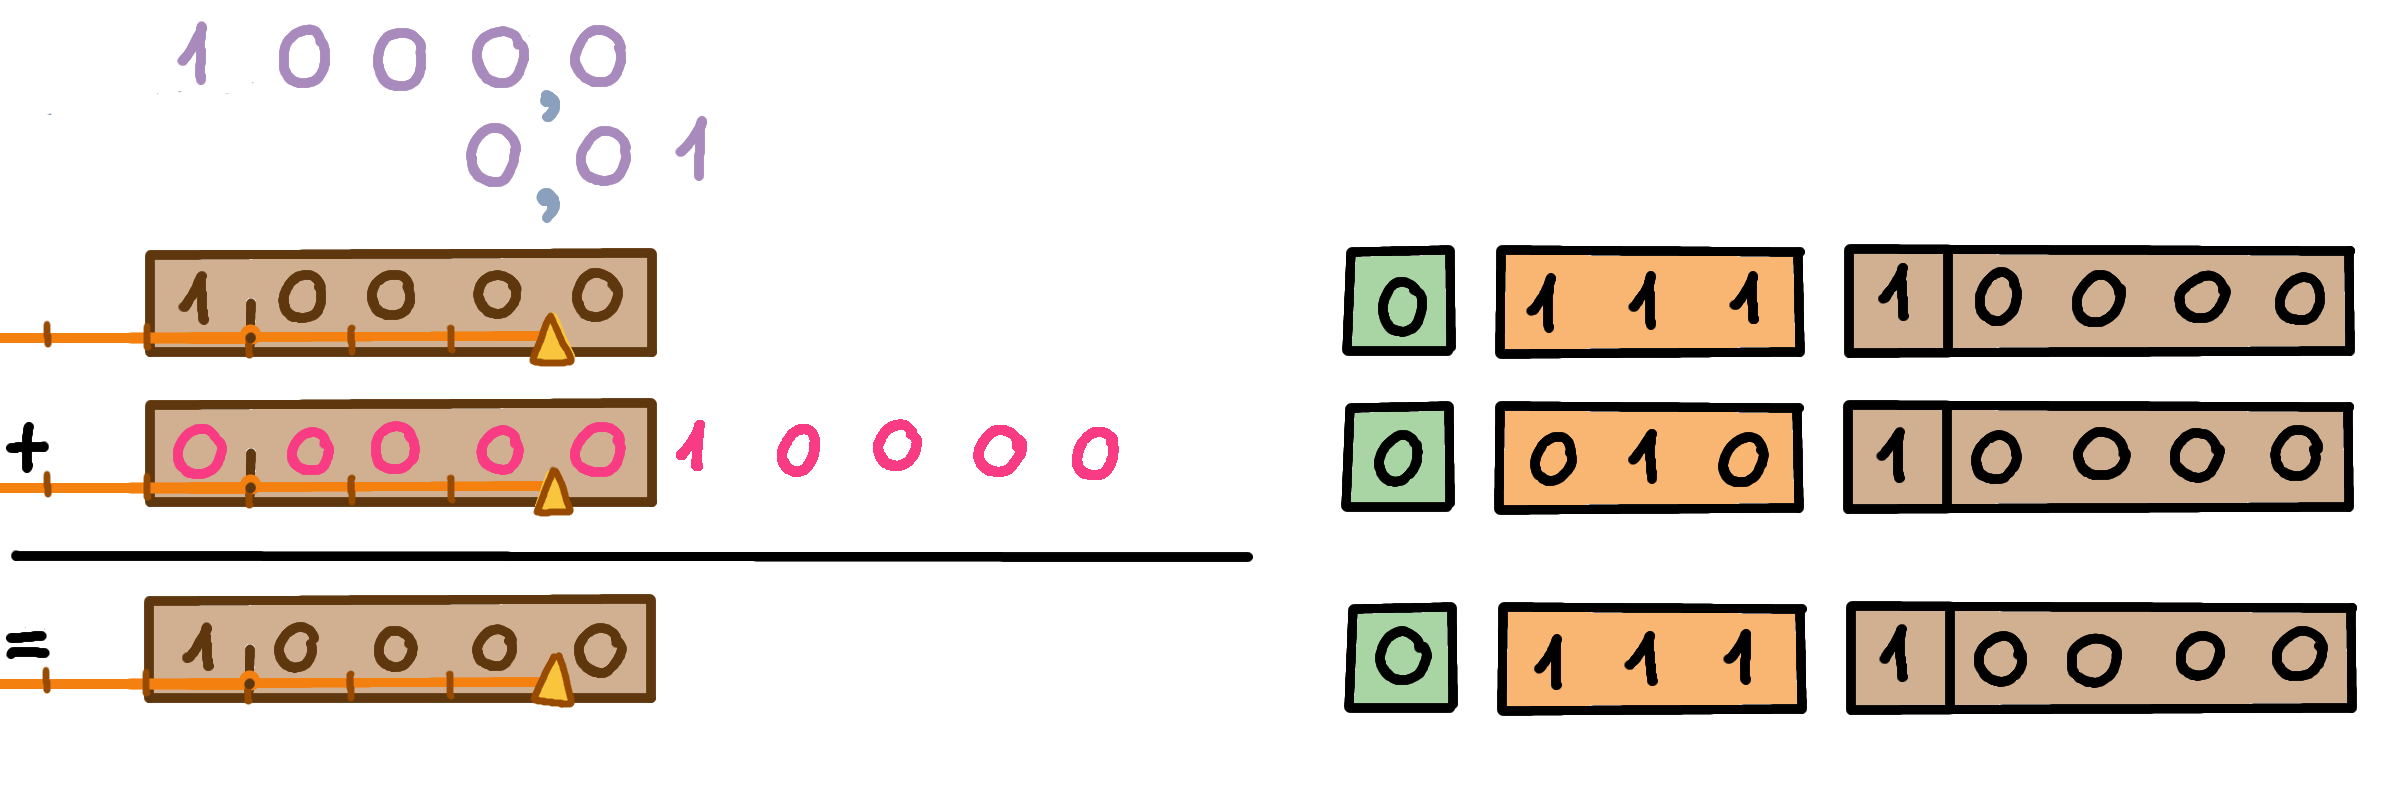
\includegraphics[width=\linewidth]{Pictures/Addition8and1-4_3.png} 
\end{figure}